\chapter{Mass Transport -- C-Processes}

\input{C/theory5}

%=========================================================================
%\section{Reactive transport}

%-------------------------------------------------------------------------
\section{Solute transport with decay}
\label{sec:decay}

\subsubsection*{Theory}

Radioactive decay is the change in the composition of a core by emitting particles and/or electro-magnetic radiation. Different kinds of radioactive decay are i.e. decay as a result of emission of negatrons or positrons and decay under emission of $\gamma$-rays.

\begin{tabbing}
\=xxxxxxxxxxxxxxxxxxxxxxx \=xxxxxxxxxxxxxxxxx \kill
\> $\alpha$-decay
\> ${^{232}_{\phantom{2}90}}\mathrm{Th}\rightarrow\;{^{228}_{\phantom{2}88}}\mathrm{Ra}+{^{4}_{2}}\mathrm{He}$ \\[1.5ex]
\> $\beta$-decay
\> ${^{228}_{\phantom{2}88}}\mathrm{Ra}\rightarrow\;{^{228}_{\phantom{2}89}}\mathrm{Ac}+{^{\phantom{-}0}_{-1}}\mathrm{e}$ \\[1.5ex]
\> $\gamma$-decay
\> ${^{236}_{\phantom{2}92}}\mathrm{U}^{\star}\rightarrow\;{^{236}_{\phantom{2}92}}\mathrm{U}+\gamma$
\end{tabbing}

The above given examples show that the radioactive decay is an irreversible process. The following differential equation describes the decay as first order reaction (without chain development):
\begin{equation}
\frac{\partial C}{\partial t}\,=\,-\lambda\cdot C
\label{eq55}
\end{equation}
{\small
with $\lambda$ - decay rate (s$^{-1}$).
}

The integration of this equation causes an exponential decay term in the following form.
\begin{equation}
C(t)\,=\,C_0\cdot e^{-\lambda\cdot t}
\label{eq56}
\end{equation}
{\small
with $C_0$ - initial concentration (kg$\cdot$m$^{-3}$).
}

The decay values are commonly expressed as the so-called half life ($t_{1/2}$). This is the point of time when half of the substance is degraded. The relation between the half-life $T$ and the decay rate results from:
\begin{equation}
e^{-\lambda\cdot t}\,=\,\frac{1}{2}\;\Rightarrow\;
\lambda\,=\,\frac{\ln(2)}{T}\,\cong\,\frac{0.693}{T}
\label{eq57}
\end{equation}


\subsubsection*{Problem definition}

The aim of this example is to simulate the mass transport with the influence of decay, but without any sorption. At the left side of the considered aquifer there is a volume source of 0.1~m$^3$/d, at the right side there is a constant water pressure of 20 kPa. The tracer substance in the source volume is distributed by a stationary flow in the homogeneous aquifer. The mass distribution after 100 days has to be calculated. Figure \ref{fig51} shows a sketch of the calculation area.

\begin{figure}[htbp]
\centering
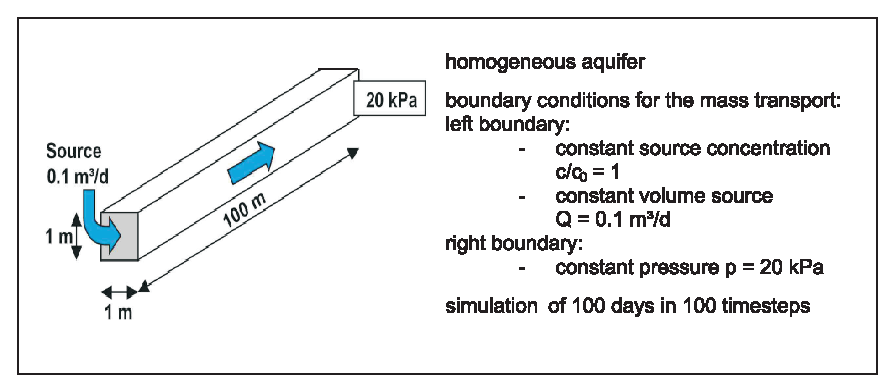
\includegraphics[width=1.0\textwidth]{C/figures/fig51.eps}
\caption{Calculation area: homogeneous aquifer}
\label{fig51}
\end{figure}

\textsl{Assumptions}

\begin{tabbing}
Component: \= no sorption, exclusively decay \\
Aquifer: \> homogeneous, saturated, stationary flow \\
\end{tabbing}

\subsubsection*{Model set-up of the 1~D numerical model}

For the 1-dimensional calculation the calculation area is simplified as a line of a length of 100~m with 100 elements and 101 nodes. As boundary conditions the relative concentration amounts 1 and the source volume of the fluid phase with 0.1~m$^3$/d is given at the left border of the calculation area and a constant pressure of 20 kPa at the right boundary. The used parameters of the soil are listed in table \ref{tab51}. The calculation is divided into 100 time steps with a constant time step length of 1 day. That means, the flow and transport processes in the aquifer within 100 days are simulated.

\begin{table}[htbp]
\centering
\begin{tabular}{|l|l|l|}
\hline
parameter & value & unit \\
\hline
porosity $\Phi$  & 0.2 &  --  \\			
\hline
permeability $K$ & 1.0$\cdot 10^{-12}$ & m$^2$ \\
\hline
density water $\rho$ & 1000 & kg$\cdot m^3$ \\
\hline
viscosity water $\eta$ & 0.001 & Pa$\cdot s$ \\
\hline
dispersion length $\alpha_l$ & 5.0 & m \\
\hline
decay in solved phase $\lambda$ & 2.0$\cdot 10^{-7}$ & s$^{-2}$ \\
\hline
\end{tabular}
\caption{Used parameters}
\label{tab51}
\end{table}

\subsubsection*{Evaluation method}
The concentration distribution at a special point in time and over a given distance is calculated by equation \ref{eq53}. Hereby the retardation coefficient is set equal to 1. The analytical solutions are depicted in figure \ref{fig52} as single symbols.

\subsubsection*{Results}

In figure \ref{fig52} you can find the concentration distribution over the whole length of the 1~D model at the final simulation time of 100 days. Obviously, the numerical results meet well the analytical solutions.

\begin{figure}[htbp]
\centering
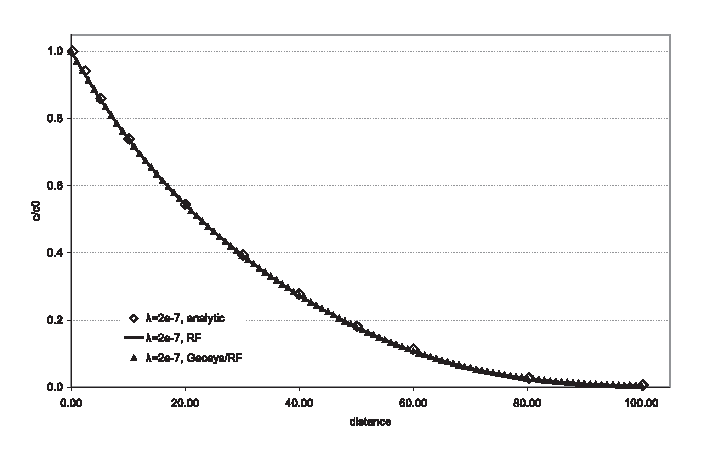
\includegraphics[width=0.8\textwidth]{C/figures/fig52.eps}
\caption{Concentration distribution after 100~d (decay)}
\label{fig52}
\end{figure}

\begin{tabular}{|l|l|l|}
\hline
Benchmark & Problem type	& Path in benchmark deposit \\
\hline	
hc\_decay\_1Du	& HC	& benchmarks $\backslash$HC$\backslash$decay \\
\hline	
\end{tabular}



%-------------------------------------------------------------------------
\section{Solute transport with sorption}

\subsubsection*{Theory}

Exchange processes, like sorption, between the solid and the liquid phase in the multiphase system of an aquifer can be caused by physical (Van-der-Waals-forces) or chemical bonds. Sorption processes can be reversible (adsorption-desorption) if the chemical environment is changing. When the transport in a multiphase system is simulated, the mass exchange between the liquid and the solid phase has to be included. The equations that describe the sorption processes are called sorption isotherms. Sorption isotherms describe the relation between the substance that is adsorbed on the solid matrix and the one which is dissolved in the fluid phase. Those equations are only valid under isothermal conditions. The isotherms that are listed below, base on the assumption that the adsorbed substance and the dissolved one are in the state of equilibrium.

\begin{eqnarray}
\mathrm{Henry:}
& \qquad &
S\,=\,K_D\cdot C \\[2.0ex]
\label{eq58}
%
\mathrm{Freundlich:}
& \qquad &
S\,=\,K_1\cdot C^{K_2} \\[2.0ex]
\label{eq59}
%
\mathrm{Langmuir:\hspace*{0.8ex}}
& \qquad &
S\,=\,\frac{K_1\cdot C}{1+K_2\cdot C}
\label{eq510}
\end{eqnarray}

{\small
with
\begin{tabbing}
\=xxxxxxxxxxxx \=xxxxxxxxxxxxxxxxxx \kill
\> $K_D,\; K_1,\; K_2$ \> - distribution coefficients, \\[1.0ex]
\> $S$ \> - concentration of the adsorbed species (kg/kg), \\[1.0ex]
\> $C$ \> - concentration of the dissolved species (kg/m$^3$).
\end{tabbing}
}

The distribution coefficients are dependent on the substance and the specific soil properties like the pH. The linear Henry-isotherm is often used when there are low concentrations. Non-linear sorption processes are reproduced by the Freundlich or the Langmuir isotherm. Then the retardation is dependent on the solute concentration. In addition, the use of the Langmuir isotherm assumes a constant amount of sorption space at the solid surface. A maximum concentration for the adsorbed substance on the solid matrix is exclusively considered by the Langmuir isotherm (Habbar, 2001). This maximum concentration $c_{\mathrm{max}}$ is included in the distribution coefficient $K_1$ ($K_1=c_{\mathrm{max}}\cdot K_2$). The distribution coefficient $K_2$ of the Langmuir isotherm stands for the affinity between solid and sorbed solute. The distribution coefficients do not have comparable values: each sorption isotherm has to be considered separately with its specific constants.


\subsection{Sorption with linear isotherm (Henry isotherm)}

\subsubsection*{Problem definition}

The aim of this example is to simulate the solute transport in an aquifer by convection with the influence of retardation as a result of sorption. The solute transport is influenced by linear sorption processes. That means, the Henry-isotherm is relevant to calculate the solute concentration. The calculation area and boundary conditions are the same as described for the precedent example.

\textsl{Assumptions}

\begin{tabbing}
Component: \= exclusively linear sorption (Henry isotherm), no decay \\
Aquifer: \> homogeneous, saturated, stationary flow \\
\end{tabbing}

\subsubsection*{Model set-up of the 1~D numerical model}

See chapter \ref{sec:decay}.

The soil parameters are the same as listed in table \ref{tab51}, but decay is not considered during these simulation runs. For the different simulation runs the Henry-sorption coefficients are varied as listed in table \ref{tab52} in order to evaluate the influence of sorption on the mass transport. The retardation coefficients R are calculated by solving equation \ref{eq52}.

\begin{table}[htbp]
\centering
\begin{tabular}{|l|l|}
\hline
K$_D$-value [m$^3$/kg] & retardation coefficient [-] \\
\hline
0  & 1  \\			
\hline
6.8 $\cdot 10^{-6}$ & 1.05 \\
\hline
6.8 $\cdot 10^{-5}$ & 1.54  \\
\hline
6.8 $\cdot 10^{-4}$ & 6.44  \\
\hline
\end{tabular}
\caption{Variation of K$_D$-values and retardation coefficients as input variables}
\label{tab52}
\end{table}

\subsubsection*{Evaluation method}

The concentration distribution at a special point in time and over a given distance is calculated by equation \ref{eq53}. Hereby the decay term $\gamma$ is set equal to 1. The analytical solutions are depicted in figure \ref{fig53} as single symbols.

\subsubsection*{Results}

In figure \ref{fig53} you can find the concentration distribution over the whole length of the 1~D model at the final simulation time of 100 days. Obviously, the numerical results meet well the analytical solutions.


\begin{figure}[htbp]
\centering
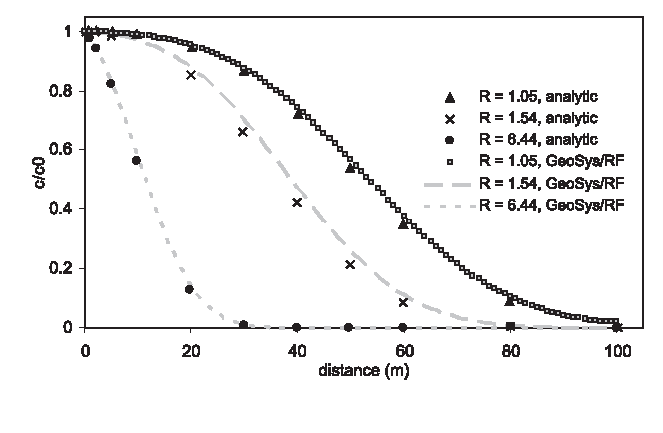
\includegraphics[width=0.8\textwidth]{C/figures/fig53.eps}
\caption{Concentration distribution after 100~d (Henry sorption)}
\label{fig53}
\end{figure}

\begin{tabular}{|l|l|l|}
\hline
Benchmark & Problem type	& Path in benchmark deposit \\
\hline	
hc\_sorp\_henry\_1D	& HC	& benchmarks $\backslash$HC$\backslash$Sorption$\backslash$Henry \\
\hline	
\end{tabular}


\subsection{Non-linear sorption with Freundlich isotherm}

\subsubsection*{Problem definition}

The non-linear Freundlich isotherm is often used to describe real sorption processes. Therefore, in this example, the transport process by including the Freundlich isotherm is calculated in the same way as in the precedent example (same model and boundary conditions). As there exists no opportunity to calculate analytically the solute transport with non-linear sorption, the results of the simulation have to be compared with solutions of the transport equation with linear sorption in order to evaluate the simulation results.

\textsl{Assumptions}

\begin{tabbing}
Component: \= non-linear sorption (Freundlich isotherm), no decay \\
Aquifer: \> homogeneous, saturated, stationary flow \\
\end{tabbing}

\subsubsection*{Model set-up of the 1~D numerical model}

See chapter \ref{sec:decay}

The soil parameters are the same as listed in table \ref{tab51}(except decay). For the different simulation runs the Freundlich-sorption coefficients (K$_1$) are varied in the same way as the K$_D$-values that are listed in table \ref{tab53}. The exponent K$_2$ was constant with a value of 1.

\subsubsection*{Evaluation method}
The dependence of sorbed molecules on the amount of molecules in dilution is given by equation \ref{eq59}. The concentration distribution at a special point in time and over a given distance cannot be calculated analytically by equation \ref{eq53} when a non-linear sorption process is assumed. A possibility to test the correctness of the simulation results for transport with Freundlich sorption is to choose values of distribution coefficients in order to create a concentration distribution which is approximately linear and must therefore almost be equal to the results of transport by use of the Henry isotherm.

\subsubsection*{Results}

As the values for the Freundlich coefficients were chosen in that way, that the concentration distribution between sorbed and solute concentrations is almost linear, the results of the simulation runs have to be equal to the results that are obtained by using the linear Henry isotherm. In figure \ref{fig54} the concentration distribution of the solute over the model length of 100~m is shown. As the concentrations of the transport simulation by using the Freundlich isotherm match those of the simulation runs with linear sorption, these results for non-linear sorption are reasonable. Additionally to this test, the values for the constant K$_2$ were changed to 0.8 in order to prove a difference between linear and non-linear sorption. The results of the comparison are shown in figure \ref{fig55}. These numerical results show the effect of the application of a non-linear sorption isotherm: the higher the influence of sorption (large value of sorption coefficient K$_D$ resp. K$_1$) the higher the difference of solute concentration values between non-linear and linear sorption. However, the results for both isotherms were not evaluated quantitatively.

\begin{figure}[htbp]
\centering
\includegraphics[width=0.8\textwidth]{C/figures/fig54.EPS}
\caption{Concentration distribution after 100~d (Freundlich compared to Henry sorption)}
\label{fig54}
\end{figure}

\begin{figure}[htbp]
\centering
\includegraphics[width=0.8\textwidth]{C/figures/fig55.EPS}
\caption{Different concentration distributions after 100~d (Freundlich compared to Henry sorption)}
\label{fig55}
\end{figure}

\begin{tabular}{|l|l|l|}
\hline
Benchmark & Problem type	& Path in benchmark deposit \\
\hline	
hc\_sorp\_Freundl\_1D	& HC	& benchmarks $\backslash$HC$\backslash$Sorption$\backslash$Freundlich \\
\hline	
\end{tabular}



\subsection{Non linear sorption with Langmuir isotherm}

\subsubsection*{Problem definition}

The non-linear Langmuir isotherm is used to describe sorption processes that are restricted by a maximum concentration of sorbed molecules. In this example, the transport process by including the Langmuir isotherm is calculated in the same way as in the precedent examples for mass transport. As there exists no opportunity to calculate analytically the solute transport with non-linear sorption, the results of the simulation have to be compared with solutions of the transport equation with linear sorption in order to evaluate the simulation results.

\textsl{Assumptions}

\begin{tabbing}
Component: \= non-linear sorption with maximum concentration (Langmuir isotherm)\\
\> no decay \\
Aquifer: \> homogeneous, saturated, stationary flow \\
\end{tabbing}

\subsubsection*{Model set-up of the 1~D numerical model}

See chapter \ref{sec:decay}

The soil parameters are the same as listed in table \ref{tab51}(except decay). In order to create a Langmuir equation which has almost the same linear characteristic as the Henry equation, the Langmuir sorption coefficients, K$_1$, were varied in the same way as the Henry coefficients (K$_D$ values in table \ref{tab52}) for the different simulation runs. The K$_2$ coefficients stand for the affinity between solid and sorbed solute. Thus, the K$_2$ value can not be set equal to 0, because this would cause a transport without any sorption. When K$_2$ equals 1, there is no effect on the binding affinity. Therefore, the coefficient K$_2$ was set constant with a value of 1 in order to approximate the linear characteristic of the Henry equation (\ref{eq58}).

\subsubsection*{Evaluation method}
The dependence of sorbed molecules on the amount of molecules in dilution is given by equation \ref{eq510}. The concentration distribution at a special point in time and over a given distance cannot be calculated analytically by equation \ref{eq53} when a non-linear sorption process is assumed. Therefore, the simulation results are compared with the results for the mass transport by using the linear Henry isotherm. The non-linear Langmuir isotherm was forced to be almost linear in the way as described above. Now the results of the transport by using the Langmuir isotherm can be compared with the results that were obtained by the transport simulation with the linear Henry isotherm.

\subsubsection*{Results}

In figure \ref{fig56} the concentration distributions over the whole model length by using the linear Henry isotherm and the non-linear Langmuir isotherm are depicted. Obviously, the results for each specified distribution constant are almost equal. This result is correct, because it was provoked by the choice of the sorption coefficients.

\begin{figure}[htbp]
\centering
\includegraphics[width=0.8\textwidth]{C/figures/fig56.EPS}
\caption{Concentration distribution after 100~d (Langmuir compared to Henry sorption)}
\label{fig56}
\end{figure}

In order to show that the results by the use of the Langmuir isotherm are actually different to those by using the Henry isotherm, the K$_2$ values were changed to a value of 0.8, so that the Langmuir isotherm got a real non-linear gradient. As the results show (fig. \ref{fig57}), the differences between the concentration distributions are evident.

\begin{figure}[htbp]
\centering
\includegraphics[width=0.8\textwidth]{C/figures/fig57.EPS}
\caption{Different concentration distributions after 100~d (Langmuir compared to Henry sorption)}
\label{fig57}
\end{figure}

\begin{tabular}{|l|l|l|}
\hline
Benchmark & Problem type	& Path in benchmark deposit \\
\hline	
hc\_sorp\_langmuir\_1D	& HC	& benchmarks $\backslash$HC$\backslash$Sorption$\backslash$Langmuir \\
\hline	
\end{tabular}


%-------------------------------------------------------------------------
\subsection{Solute transport with sorption and decay}

\subsubsection*{Problem definition}

The aim of this example is to simulate the solute transport in an aquifer by convection with the influence of retardation as a result of sorption. Additionally, the transported mass will be degraded. The calculation area and boundary conditions are the same as described in chapter \ref{sec:decay}.


\textsl{Assumptions}

\begin{tabbing}
Component: \= linear sorption, decay \\
Aquifer: \> homogeneous, saturated, stationary flow \\
\end{tabbing}

\subsubsection*{Model set-up of the 1~D numerical model}

See chapter \ref{sec:decay}

The soil parameters are the same as listed in table \ref{tab51}. The decay rate $\lambda$ is 2$\cdot 10^{-7}$~s$^-1$. For the different simulation runs the Henry sorption coefficients are varied as listed in table \ref{tab52} to evaluate again the influence of sorption on mass transport.

\subsubsection*{Evaluation method}
The concentration distribution at a special point in time and over a given distance is calculated by equation \ref{eq53}. The analytical solutions are depicted in figure \ref{fig58} as single symbols.

\subsubsection*{Results}

The influence of radioactive decay on the transport process can be recognised at the typical declining exponential curves in figure \ref{fig58}. According to the different sorption coefficients the transport is retarded. Obviously, the numerical results (lines) meet well the analytical solutions. Therefore, it can be summarised that the transport under the combined consideration of both decay and sorption can be reproduced by the simulation with RockFlow.

\begin{figure}[htbp]
\centering
\includegraphics[width=0.8\textwidth]{C/figures/fig58.EPS}
\caption{Concentration distributions after 100~d (sorption and decay)}
\label{fig58}
\end{figure}

\begin{tabular}{|l|l|l|}
\hline
Benchmark & Problem type	& Path in benchmark deposit \\
\hline	
hc\_decay\_sorp\_henry\_1Du	& HC	& benchmarks $\backslash$HC$\backslash$sorption\_decay \\
\hline	
\end{tabular}


%-------------------------------------------------------------------------
%\subsection{Multi component transport}

%\subsubsection*{Problem definition}

The aim of this example is to simulate the transport of several components with different sorption behaviour and decay. The calculation area and boundary conditions are the same as described for the precedent example. The mass distribution after 100 days has to be calculated.

\textsl{Assumptions}

\begin{tabbing}
Component 1: \= no sorption, no decay \\
Component 2: \> decay \\
Component 3: \> linear sorption \\
Component 4: \> linear sorption, decay \\
Aquifer: \> homogeneous, saturated, stationary flow \\
\end{tabbing}

\subsubsection*{Model set-up of the 1~D numerical model}

See chapter \ref{sec:decay}

The soil parameters are the same as listed in table \ref{tab51}. The decay rate $\lambda$ for components 2 and 4 is 2$\cdot 10^{-7}$~s$^-1$, the Henry sorption coefficient K$_D$ for component 3 is 6.4$\cdot 10^{-4}$~kg/m$^-3$ (R = 6.44).

\subsubsection*{Evaluation method}
The concentration distribution at a special point in time and over a given distance is calculated by equation \ref{eq9}. The analytical solutions are depicted in figure \ref{fig59} as single symbols.

\subsubsection*{Results}

In figure \ref{fig59} you can find the concentration distribution of the 4 different components over the whole length of the 1D-model at the final simulation time of 100 days. As the comparison of each single component with the analytical results of the "one-component-transport" shows, the numerical results for the multi component transport are reasonable.

\begin{figure}[htbp]
\centering
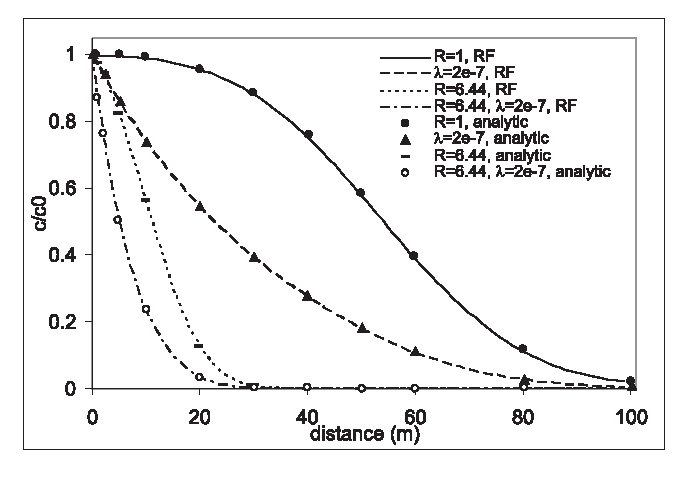
\includegraphics[width=0.5\textwidth]{C/figures/fig59.eps}
\caption{Concentration distributions of the four components after 100~d}
\label{fig59}
\end{figure}


\begin{tabular}{|l|l|l|l|}
\hline
Path in the & Used code	& Used version & Date of si- \\
benchmark deposit	& & & mulation run \\
\hline
$\backslash$HC$\backslash$multi\_component$\backslash$ &Rockflow	& RockFlow 5,	& Mar. 2007 \\
hc\_multi-c\_1D.rfd/rfi	&  & rf\_gui1407-rf5065 & \\
\hline	
\end{tabular}


%-------------------------------------------------------------------------
\section{Solute transport by diffusion}


\textbf{Theory}

Diffusion is a process that equates concentration differences of gaseous or dissolved matter or energy. The particles move from higher to lower concentrations by Brownian movement in dependence on the temperature. In an aquifer, diffusive transport appears when convective transport is not that relevant (small velocities).

The extent of diffusion is also dependent on the diffusing substance and the medium. In addition, diffusion in soils is influenced by other factors, e.g. tortuosity. The finer a soil the stronger are the interacting forces between the soil matrix and the diffusing molecules. The diffusion coefficient which has to be given in GeoSys/RockFlow is the so-called apparent diffusion coefficient (eq. \ref{eq511}).
\begin{equation}
D_a\,=\,\frac{D_e}{\Phi}
\label{eq511}
\end{equation}
{\small
with $D_e$ - effective diffusion coefficient.
}


\subsection{Diffusion: axisymmetric model}


\subsubsection*{Problem definition}

This diffusion model is built to reproduce a field study in clay. This in situ test consists of a borehole where a solution is circulated that contains tracer substances like HTO. These tracers diffuse into the adjacent clay. The aim of the investigation is to simulate the HTO distribution after 300 d, the final test time, and to compare the simulation results of GeoSys/RockFlow to those that are calculated by HYDRUS 1~D (Simunek et al.) and PHAST (Parkhurst et al.).

\subsubsection*{Model set-up of the 1~D axisymmetric model}

To build a proper model of the tracer test, a one-dimensional axisymmetric model with 3.8~cm of borehole radius and 21.2~cm horizontal distance in the clay soil is created. As initial condition a constant pressure of 0 was specified in the whole model and the concentration relation c/c$_0$ of 1 within the distance of the borehole radius and of 0 within the clay domain. The pressure boundary condition corresponds to the initial condition. The calculation model includes 310 elements and 311 nodes. Table \ref{tab53} shows the used parameters for the clay and the apparent diffusion constant D$_a$ of HTO. The calculation is performed for the test duration of 300 days with fitted time step lengths from 0.001~d to 1~d (Bahr, 2007). The porosity in the modelled borehole is assumed to be 1 in order to evoke the simulation of a tracer reservoir that supplies the tracer solution into the clay.

\begin{table}[htbp]
\centering
\begin{tabular}{|l|l|l|}
\hline
parameter & value & unit \\
\hline
density $\rho$  & 2.5 & t $\cdot$ m$^{-3}$  \\			
\hline
porosity $\Phi$ & 0.15 & -- \\
\hline
permeability $K$ & 1.0$\cdot 10^{-11}$ & m$^2$ \\
\hline
diffusion coefficient D$_a$ & 3.6$\cdot 10^{-10}$ & m$^2\cdot s^{-1}$  \\
\hline
\end{tabular}
\caption{Parameters}
\label{tab53}
\end{table}

\subsubsection*{Evaluation method}
The aim of the presented calculation example is the evaluation of the GeoSys/RockFlow-simulation results by comparing them with numerical results of two other simulation programmes. The comparison is made by the use of Hydrus 1~D, which is a one-dimensional transport model especially for the solute transport in soils. The second programme, PHAST, is linked to the chemical software PHREEQC. The simulation with both programmes was made under consideration of the same boundary conditions and parameters (Bahr, 2007).

\begin{figure}[htbp]
\centering
\includegraphics[width=0.8\textwidth]{C/figures/fig510.EPS}
\caption{Concentration distributions after 300~d}
\label{fig510}
\end{figure}

\subsubsection*{Results}

In figure \ref{fig510} you can find the concentration distributions over the width of 0.25~m after a simulation time of 300 days that were calculated by means of GeoSys/RockFlow, PHAST and Hydrus 1D (Bahr, 2007). The numerical results accord well to each other. Thus, the comparison shows that the diffusion process can be well reproduced by the use of an axisymmetric GeoSys/RockFlow model.

\begin{tabular}{|l|l|l|}
\hline
Benchmark & Problem type	& Path in benchmark deposit \\
\hline	
Diff\_HTO\_test	& HC	& benchmarks $\backslash$HC$\backslash$Diffusion$\backslash$ \\
\hline	
\end{tabular}


\subsection{Diffusion in an anisotropic medium (2~D simulation)}


\subsubsection*{Problem definition}

The aim of this example is to simulate the transport of a tracer by molecular diffusion in an anisotropic porous medium. The side length of the square numerical model is 1~m. At the left corner at the bottom of the model a constant concentration is diffusing into the calculation area. Diffusion is the only process for tracer transport, there are no pressure differences in the whole area. Because of the anisotropy of the soil material the tracer has to diffuse much faster in x-direction than in vertical direction. This has to be evaluated by comparing the concentration distributions in both directions.

\subsubsection*{Model set-up of the 2~D numerical model}

As initial condition the pressure and tracer concentration were set to 0 in the whole area. At the left corner at the bottom of the model a concentration relation c/c$_0$ of 1 is specified along two polylines of the length of 0.3~m. The boundary conditions correspond to the initial conditions. The calculation model includes 736 triangular elements and 409 nodes. Table \ref{tab55} shows the used parameters for the simulation. As the porous medium is assumed to be anisotropic, which influences diffusion, the value for tortuosity is set equal to 1 in x-direction and 0.1 in y-direction.

\begin{table}[htbp]
\centering
\begin{tabular}{|l|l|l|}
\hline
parameter & value & unit \\
\hline
porosity $\Phi$ & 0.4 & -- \\
\hline
permeability $K$ & 1.0$\cdot 10^{-15}$ & m$^2$ \\
\hline
density water $\rho$  & 1000 & kg/m$^{-3}$  \\		
\hline	
viscosity water $\eta$ & 0.001 & Pa$\cdot$ s \\
\hline	
dispersion length & 10.0 & m \\
\hline
diffusion coefficient D$_a$ & 6.0$\cdot 10^{-10}$ & m$^2$/s  \\
\hline
\end{tabular}
\caption{Used parameters}
\label{tab55}
\end{table}

The calculation is made for 30 time steps with a length of 1$\cdot$10$^7$ seconds. The calculation model is sketched in figure \ref{fig511}.

\begin{figure}[htbp]
\centering
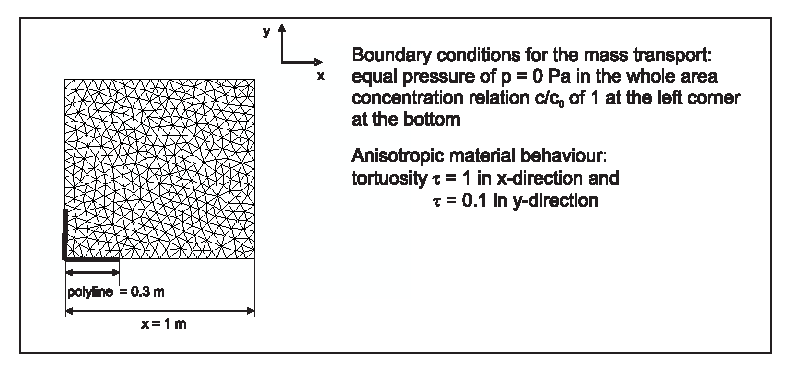
\includegraphics[width=0.9\textwidth]{C/figures/fig511.eps}
\caption{Calculation model (2D)}
\label{fig511}
\end{figure}

\subsubsection*{Evaluation method}
As the process of diffusion is dependent on the actual concentration in the porous medium and on the point in time, an analytical solution for the present calculation model is not possible. Therefore, the results of the RockFlow simulation are solely evaluated in a qualitative way by comparing the concentration distributions in horizontal and vertical direction.

\begin{figure}[htbp]
\centering
\includegraphics[width=0.8\textwidth]{C/figures/fig512.EPS}
\caption{Concentration distributions in x- and y-direction}
\label{fig512}
\end{figure}

\subsubsection*{Results}

In figure \ref{fig512} you can find the concentration distributions over the model side length of 1~m in x- and y-direction, respectively, after a simulation time of 1$\cdot$10$^8$ seconds. Assuming a small tortuosity of 0.1, the component is not yet transported over the whole transport length of 1~m in vertical direction, while in horizontal direction the concentration relation equals approximately 0.3 at the opposite border of the model. The shown trend in the change of diffusion velocity by assuming different tortuosities in x- and y-direction in order to specify anisotropic material behaviour for molecular diffusion has a comprehensible characteristic.

\begin{tabular}{|l|l|l|}
\hline
Benchmark & Problem type	& Path in benchmark deposit \\
\hline	
diff\_aniso	& HC	& benchmarks $\backslash$HC$\backslash$Diffusion$\backslash$ \\
\hline	
\end{tabular}


\subsection{Solute transport with matrix diffusion}
\subsubsection*{Problem definition}
This benchmark is introduced to verify the matrix diffusion function
developed by Chris McDermott and Georg Kosakowski. It simulates
advective -dispersive transport of a solute in an one-dimensional
fracture with constant aperture, with and without the effect of
matrix-diffusion. The geometry and the material parameters are
chosen to fit the parameters extracted from experiments conducted
during the Colloid Radionuclide Retardation Experiment at Nagra's
Grimsel test site \ref{KosaSmith:2005}. The result from GS/RF is
compared with that from PICNIC, and they fit well.

\subsubsection*{Model set-up of the 1D domain}
\begin{figure}[!htb]
  \begin{center}
    \includegraphics[scale=0.25]{C/figures/fig_matdiff_domain.eps}
  \end{center}
  \caption{Conceptual setup of the 1D problem}
  \label{c:matdiff_dom}
\end{figure}
The geometry and material parameters in PICNIC and GS/RF are
summarized in Table \ref{tab:c_matdiff_setting} and the conceptual
model is shown in Figure \ref{c:matdiff_dom}. PICNIC solves the
one-dimensional problem, whereas in GS/RF a two-dimensional
discretization was chosen. A rectangular domain of 5.2m $\times$
0.5m was discretized with 1155 nodes and 2080 triangular elements.
One of the shorter domain edges was chosen as inflow boundary and
fluid was injected at the boundary-nodes in such a way, that the
resulting fluid velocity matches exactly the value from
\ref{tab:c_matdiff_setting}. The concentration is fixed at the
inflow boundary. In 2.5m distance the breakthrough curve is
recorded. The outflow boundary is assumed to be far away and should
not influence the observed breakthrough curve.Picnic V2.2 and GS/RF
Rev. 1535 from the subversion server were used for testing.

As defining exactly the same transport boundary conditions in GS/RF
and PICNIC is not possible, the following procedure was used to get
the inflow boundary condition as similar as possible:

1) The system was calculated for injecting a pulse of solute with a
constant flux for a time length of 50s with PICNIC. The
concentration vs. time was recorded for the inflow-leg.

2) The concentrations vs. time extracted from PICNIC's inflow-leg
were applied (fixed) to the inflow boundary of the GS/RF system.

These procedures work, as long as advective fluxes are much higher
than the dispersive-diffusive fluxes over the boundary.

The outflow boundary condition is set to infinity, i.e. a
semi-infinite problem is calculated. In GS/RF the domain is set to
5m, double the distance between inflow boundary and observation
point. This prevents the outflow boundary condition to influence the
tracer breakthrough at the observation point.

\begin{table}[H]
  \begin{center}
  \begin{tabular}{llll}
\hline\noalign{\smallskip}
  \hline
 Symbol & Unit & Description & Value \\
  \hline
 $L$ & $m$ & Distance between boundary and observation points & $2.5$ \\
 $\alpha_{T}$ & $m$ & Trans. dispersion (GS/RF only) & $-$ \\
 $\rho$ & $kg/m^{3}$ & Bulk matrix density & $2670$ \\
 $2b$ & $m$ & Fracture aperture & $0.55\times10^{-3}$ \\
 $v$ & $m/s$ & Fluid velocity & $7.05\times10^{-4}$ \\
 $\alpha_{L}$ & $m$ & Long. dispersion (GS/RF only) & $0.1$ \\
 $Pe$ & $-$ & Peclet number (PICNIC only) & $25$ \\
 $\varepsilon_{p}$ & $-$ & Matrix porosity & $0.3$ \\
 $D_{p}$ & $m^{2}/s$ & Diffusion constant in rock matrix & $7.4\times10^{-11}$ \\
  \hline
  \hline
  \end{tabular}
  \caption{Geometry and material properties for the simulations} %\footnotesize
  \label{tab:c_matdiff_setting}
  \end{center}
\end{table}

\subsubsection*{Results}
For the investigated two cases, advection and dispersion(ADE) only
and ADE plus matrix diffusion(MD), the PICNIC and GS/RF solutions
are in general very similar (see Figure \ref{c:matdiff_result}).

\begin{figure}[!htb]
  \begin{center}
  \includegraphics[scale=0.5]{C/figures/fig_matdiff_result.eps}
  \end{center}
  \caption{Breakthrough of the ADE and the ADE+MD solutions calculated with PICNIC and GS/RF}
  \label{c:matdiff_result}
\end{figure}

\begin{tabular}{|l|l|l|}
  \hline
  Benchmark & Problem type & Path in benchmark deposit \\
  \hline
 \emph{matrix\_diffusion} & C & benchmarks\verb \C\matrix_diffusion\OGS_vs_picnic \\
  \hline
\end{tabular}



\subsection{Solute transport with cation exchange}


\subsubsection*{Theory}

In contrast to sorption the ion exchange is the replacement of one chemical for another one at the solid surface, the so called ion exchanger. Ion exchange equations do explicitly account for all ions which compete for the exchange sites. The exchange of ions is limited by the exchange capacity, which is the sum of exchangeable ions in the soil and fluctuates with the change of pH in the soil solution. The ion exchanger can be unselective or can have binding preferences for certain ions or classes of ions, depending on their chemical structure (Appelo and Postma, 1996). 

\subsubsection*{Problem definition}

This test example is taken from the PHREEQC User's Guide (Parkhurst and Appelo, 1999), a manual for a computer program that is applicable for chemical reactions and transport processes. The simulation is made in order to reproduce the transport of solutes by saturated flow with the influence of cation exchange. The aim of the example is to check out the correctness of the coupling between GeoSys/RockFlow and PHREEQC by comparing the results of the simulations of both programs. With the calculation model the chemical composition of the effluent from a column containing a cation exchanger and a sodium-potassium-nitrate-solution is simulated. This column is flushed with 3 pore volumes of calcium chloride solution.

\textsl{Assumptions}

\begin{tabbing}
Components: \= calcium, potassium and sodium react to equilibrium with cation \\ \>exchanger at all times \\
Aquifer: \> homogeneous, saturated, stationary flow \\
\end{tabbing}

\subsubsection*{Model set-up of the 1~D numerical model}

The 8.2~cm long column contains a sodium-potassium-nitrate solution that is in equilibrium with a cation exchanger. For the one-dimensional calculation the calculation area is simplified as a line of a length of 8.2~cm. The calculation model includes 82 elements and 83 nodes. As initial condition the water head in the whole domain is given with 2~m. The initial state of the solution is given in table \ref{tab56}.

\begin{table}[htbp]
\centering
\begin{tabular}{|l|l|l|}
\hline
parameter & value & unit \\
\hline
Ca & 0 & -- \\
\hline
Cl & 0 & -- \\
\hline
K & 2.0$\cdot 10^{-4}$ & mol/kgw \\
\hline
Na & 1.0$\cdot 10^{-3}$ & mol/kgw \\
\hline
N(5) & 1.2$\cdot 10^{-3}$ & mol/kgw \\
\hline
pH & 7 & -- \\
\hline
pe & 12.5 & -- \\
\hline
Na-X & 5.493$\cdot 10^{-4}$ & mol/kgw \\
\hline
K-X & 5.507$\cdot 10^{-4}$ & mol/kgw \\
\hline
Ca-X$_2$ & 0 & -- \\
\hline
\end{tabular}
\caption{Used parameters}
\label{tab56}
\end{table}

{\small
with
\begin{tabbing}
\=xxxxxxx \=xxxxxxxxxxxxxxxxxx \kill
\> pe \> - redox potential \\
\> X \> - ion exchanger \\
\> kgw \> - kilogram of water. \\
\end{tabbing}
}

At the right border of the model the constant head is given with 2~m. At the left border a constant flux of 1.388$\cdot 10^{-6}$~m$^3$/s is defined as source term. The concentrations of this infiltrating CaCl$_2$-solution as well as the pH and pe are given in table \ref{tab57}.

\begin{table}[htbp]
\centering
\begin{tabular}{|l|l|l|}
\hline
parameter & value & unit \\
\hline
Ca & 6.0$\cdot 10^{-4}$ & mol/kgw \\
\hline
Cl & 1.2$\cdot 10^{-3}$ & mol/kgw \\
\hline
pH & 7 & -- \\
\hline
pe & 12.5 & -- \\
\hline
\end{tabular}
\caption{State of the infiltration solution}
\label{tab57}
\end{table}

The soil material is specified by the parameters in table \ref{tab58}. The dispersion of the transported solutes in this soil is set equal to 2$\cdot 10^{-3}$~m. The calculation is divided in 480 time steps with a constant time step length of 180 seconds. That means, the flow and transport processes in the aquifer within 1 day are simulated.

\begin{table}[htbp]
\centering
\begin{tabular}{|l|l|l|}
\hline
density $\rho$  & 2000 & kg/m$^{-3}$  \\
\hline
porosity $\Phi$ & 0.5 & -- \\
\hline
permeability $K$ & 1.157$\cdot 10^{-5}$ & m$^2$ \\
\hline
\end{tabular}
\caption{Soil parameters}
\label{tab58}
\end{table}

\subsubsection*{Evaluation method}
As this test example has the aim to validate the coupling of GeoSys/RockFlow and PHREEQC, merely the comparison between the simulation results of both programs has to be accomplished.


\begin{figure}[htbp]
\centering
\includegraphics[width=0.8\textwidth]{C/figures/fig513.EPS}
\caption{Effluent concentrations  with time of the GeoSys/RockFlow and PHREEQC simulations}
\label{fig513}
\end{figure}

\subsubsection*{Results}

The numerical results are shown in figure \ref{fig513}. The time-dependent concentrations are the values of the compared GeoSys/RockFlow and PHREEQC models at the end node and end cell, respectively. Within the calculation time of one day the pore volume of the column model is exchanged three times. As chloride is a conservative tracer it arrives already after the exchange of about one pore volume in the effluent. As long as the exchanger contains sodium this component is eluted. Sodium is initially present in the column and exchanges with the incoming calcium. Potassium is released after sodium. When all of the potassium has been released, the concentration of calcium increases to a steady-state value. As depicted in figure \ref{fig513}, between the GeoSys/RockFlow and the PHREEQC simulation results there are no differences.

\begin{tabular}{|l|l|l|}
\hline
Benchmark & Problem type	& Path in benchmark deposit \\
\hline	
pqc1	& HC	& benchmarks $\backslash$HC$\backslash$ion\_exchange \\
\hline	
\end{tabular}


%-------------------------------------------------------------------------
\subsection{1-D Multi-component transport with dissolution and precipitation}
\subsubsection*{Problem definition}
In this example, a one-dimensional column that initially contains
calcite is continuously flushed by water that contains magnesium
chlorine (Fig. \ref{c:cal_dom}). With the movement of water front,
calcite starts to dissolve and dolomite is formed temporarily.
\begin{figure}[!htb]
  \begin{center}
    \includegraphics[scale=0.5]{C/calcite_domain.eps}
  \end{center}
  \caption{Model domain}
  \label{c:cal_dom}
\end{figure}
\subsubsection*{Media Properties}
The media properties of this model is listed in Table
\ref{tab:c_calcite_mp}.

 \begin{table}[H]
  \begin{center}
  \begin{tabular}{lrl}
\hline\noalign{\smallskip}
  \hline
 Property & Value & Unit \\
  \hline
 Column length & $0.5$ & $m$ \\
 Effective porosity & $0.32$ & $-$ \\
 Bulk density & $1.8\times10^{3}$ & $kg/m^{3}$ \\
 Longitudinal dispersivity & $0.0067$ & $m$ \\
 Pore velocity & $9.375\times10^{-6}$ & $m/sec$ \\
 Flow rate & $3\times10^{-6}$ & $m^{3}/sec$ \\
  \hline
  \hline
  \end{tabular}
  \caption{Material properties} %\footnotesize
  \label{tab:c_calcite_mp}
  \end{center}
  \end{table}

\subsubsection*{Initial and Boundary conditions}
For GS/RF-GEMIPM2K calculation, all the possible chemical species
need to be explicitly set up for initial and boundary conditions. In
this example, all concentration values are given in the unit of
$mol/kg water$. Detailed values can be get from the
*.ic and *.bc files in the corresponding benchmark folder.

\subsubsection*{Results}
This model can be simulated by GS/RF-PHREEQC, GS/RF-ChemApp, and
GS/RF-GEMIPM2K. In these benchmarks, we use the Nagra/PSI
database \cite{PSI_Database:02}, which provides same thermodynamic
data for all three calculations. Fig. \ref{c:cal_rst}
shows the three simulation results. Solid lines are for GS/RF-PHREEQC,
symbols "+" are for GS/RF-GEMIPM2K, and triangles are for GS/RF-ChemApp.

\begin{figure}[!htb]
  \begin{center}
    \includegraphics[scale=0.3]{C/calcite_result.eps}
  \end{center}
  \caption{Benchmark results from GS/RF-ChemApp, GS/RF-PHREEQC, and GS/RF-GEMIPM2K}
  \label{c:cal_rst}
\end{figure}


% \begin{figure}[!htb]
%   \begin{center}
%     \includegraphics[scale=0.3]{C/calcite_result_chemapp.eps}
%   \end{center}
%   \caption{Benchmark results from GS/RF-ChemApp}
%   \label{c:cal_chemapp}
% \end{figure}

\subsubsection*{Benchmark deposit}
\begin{tabular}{|l|l|l|}
  \hline
  Benchmark & Problem type & Path in benchmark deposit \\
  \hline
 \emph{calcite\_gems} & C & benchmarks\verb \C\calcite_gems\ \\
   \hline
 \emph{calcite\_pqc} & C & benchmarks\verb \C\calcite_pqc\ \\
  \hline
 \emph{calcite\_chemapp} & C & benchmarks\verb \C\calcite_ChemApp\ \\
  \hline
\end{tabular}

\section{1D and 2D conservative transport}


% file constrans.tex


\subsection[1D reactive transport]{1D reactive transport with comparison to analytical solution}
\label{l_s_benchmark_1d}

This benchmark describes reactive and conservative mass transport in a one-dimensional aquifer and has two aims. Firstly, a conservative component, a linearly retarded component and a component decaying according to a first order decay are transported and profiles as well as breakthrough curves are compared with the corresponding analytical solution. This comparison is possible only using these simplified reaction types. Secondly, the benchmark is set up in a way that allows to test all element types in this simplified "quasi" one-dimensional setup.

The model aquifer has a length of 100 m in x-direction and 1 m in both y and z direction. Discretization is in element sizes of 1 m in x direction, yielding 100 elements and 101 nodes for the line elements, 100 elements and 202 nodes for the quad elements, 200 elements and 202 nodes for the triangular elements, 100 elements and 404 nodes for the hexahedra elements, 200 elements and 404 nodes for the prism elements and 600 elements and 404 nodes for the tetrahedra elements. To make the boundary conditions consistent with all element types, surfaces in the y-z plane are used to define the boundary conditions at x=0 m and x=100 m.

 The hydraulic conductivity is assumed to be isotropic and constant in the whole aquifer. Flow is from the left to the right (small to large x), induced by fixed head boundary conditions at x=0 and x=100 and a total head difference of 1 m. All components have initial conditions of 0 and a constant concentration boundary condition of 1 at x=0. For the purpose of this benchmark, the concentration units are arbitrary and are therefore normalized. Transport velocity corresponds to 1 m~d$^{-1}$, thus time step length is chosen accordingly as 86400 s (corresponding to 1 d). Total simulation time is 100 d. Thus the Courant number $Co = 1.0$ and the grid Peclet number $Pe_g = 4$, keeping effects of numerical dispersion as well as oscillations sufficiently small.
 All parameters used in this simulation are given in table Tab.~\ref{l_tab_benchmark_1d}.

Three components are used in this benchmark: The component \texttt{ConsTracer} denotes the conservative tracer, for which the advection - dispersion equation is solved. Component \texttt{Decay} is transported according to the advection - dispersion equation with a first order decay rate $\lambda$. Component \texttt{SorbLin} is transported according to the advection - dispersion equation with a linear instantaneous sorption, which corresponds to a retardation of $R = 1 + \frac{1-n}{n} \rho_s K_d = 1 + \frac{0.5}{0.5} \cdot 2000 \cdot0.001 = 3$. All components have the same aqueous phase diffusion coefficient.

%\begin{figure}[htbp]
%\centering
%\includegraphics[width=0.6\textwidth]{figs/fig3_1.eps}
%\caption{Model area and Boundary conditions - adapt to actual setting}
%\label{l_fig_benchmark_1d_1}
%\end{figure}



\begin{table}[htbp]
\caption{Parameters used for benchmark HC$\backslash$1d\_analyt }
\centering
\begin{tabular}{|l|l|l|}
\hline
parameter & value & unit \\
\hline
porosity $\Phi = n $  & 0.5 &  --  \\			
\hline
hydraulic conductivity $K$ & 5.787037$\cdot 10^{-04}$ & ms$^{-1}$ \\
\hline
storage coefficient $S$ & 0.0 & s$^{-1}$ \\
\hline
solid density $\rho_s$ & 2000 &  kg$\cdot m^{-3}$ \\
\hline
density of water $\rho_w$ & 1000 & kg$\cdot m^{-3}$ \\
\hline
viscosity water $\eta$ & 0.001 & Pa$\cdot s$ \\
\hline
dispersion length $\alpha_l$ & 0.25 & m \\
\hline
component diffusion coefficient $D$ & 1.0$\cdot 10^{-9}$ & m$^2$s$^{-1}$ \\
\hline
first order decay rate in water $\lambda$ & 1.0$\cdot 10^{-7}$ & s$^{-1}$ \\
\hline
distribution coefficient $K_d$ & 1.0$\cdot 10^{-3}$ & m$^3$ kg$^{-1}$ \\
\hline
\end{tabular}
\label{l_tab_benchmark_1d}
\end{table}


\subsubsection*{Evaluation method}
Model results are compared to the analytical solution for component profiles along x after a simulation time of 75 days, as well as for breakthrough curves at x=50 m for all components. To facilitate testing of all elements, a batch-file is provided (1D\_all.bat) which reruns the benchmark for all element types by replacing the mesh file accordingly. Results can be viewed using the corresponding layout files by Tecplot. \texttt{companaProfile\_*.lay} is used for displaying the profile results and \texttt{companaBTC\_*.lay} is used for displaying the breakthrough curve results for element type \texttt{*}. The files \texttt{companalytBTC.lpk} and \texttt{companaProfile.lpk} save the simulation results for both types from an earlier GeoSys/RockFlow version for reference.


\subsubsection*{Results}

Results of the simulation and the comparison with the analytical solution are shown in Fig.~\ref{l_fig_benchmark_1d_analyt_1} for the profiles and in Fig.~\ref{l_fig_benchmark_1d_analyt_2} for the breakthrough curves. Numerical results using GeoSys/RockFlow are denoted by symbols, the analytical solution is denoted by the full lines. Correspondence is very good in both cases.

\begin{figure}[htbp]
\centering
\includegraphics[width=0.6\textwidth]{C/figures/1d_analyt_profile.eps}
\caption{Concentration profiles after 100~d}
\label{l_fig_benchmark_1d_analyt_1}
\end{figure}


\begin{figure}[htbp]
\centering
\includegraphics[width=0.6\textwidth]{C/figures/1d_analyt_btc.eps}
\caption{Concentration breakthrough curves at x=50 m }
\label{l_fig_benchmark_1d_analyt_2}
\end{figure}



\begin{table}[htbp]
\centering
\begin{tabular}{|l|l|l|}
\hline
Benchmark & Type & Path \\
\hline
\texttt{1d\_analyt}& HC &  benchmarks$\backslash$C$\backslash$1d\_analyt  \\			
\hline
\end{tabular}
\label{path}
\end{table}


\subsection[2D conservative transport]{2D conservative transport with comparison to analytical solution}
\label{l_s_benchmark_2d}

This benchmark describes the conservative mass transport in a two-dimensional homogeneous aquifer. The main purpose is to compare the numerical results of a conservative mass transport simulation without any reactions with the suitable analytical solution.

The model aquifer has a length of 100 m in the x-direction, 50 m in the y-direction and 1 m in the z direction. The whole domain is discretized into 10560 triangular elements with a constant x and y dimension of 1 m (this value guarantees a Peclet number = 4), except at the boundaries of the injection area where a finer grid is chosen.

The aquifer is assumed to have a homogeneous and isotropic hydraulic conductivity and the constant head boundary conditions on the left (piezometric surface of 2 m) and right side (piezometric surface of 1 m) produce a steady state flow in the right direction. As the material has a constant porosity of 0.5 the resulting flow velocity is 1.1574074 10$^{-3}$ m~s$^{-1}$. Both longitudinal and transversal dispersivity have a value of 0.25, consequently the total simulation time of 80 days is divided into 160 time steps to insure a Courant number lower than 1.
The constant tracer is injected with a relative concentration value of 1.0 from a source 8 m wide set on the left boundary of the aquifer, while the initial concentration of the tracer is zero all over the aquifer domain.

\begin{table}[htbp]
\caption{Parameters used for benchmark HC$\backslash$2d\_analyt }
\centering
\begin{tabular}{|l|l|l|}
\hline
parameter & value & unit \\
\hline
porosity $\Phi = n $  & 0.5 &  --  \\			
\hline
hydraulic conductivity $K$ & 5.787037$\cdot 10^{-05}$ & ms$^{-1}$ \\
\hline
storage coefficient $S$ & 0.0 & s$^{-1}$ \\
\hline
solid density $\rho_s$ & 2000 &  kg$\cdot m^{-3}$ \\
\hline
density of water $\rho_w$ & 1000 & kg$\cdot m^{-3}$ \\
\hline
viscosity water $\eta$ & 0.001 & Pa$\cdot s$ \\
\hline
longitudinal dispersivity $\alpha_l$ & 0.25 & m \\
\hline
transversal dispersivity $\alpha_l$ & 0.25 & m \\
\hline
component diffusion coefficient $D$ & 1.0$\cdot 10^{-9}$ & m$^2$s$^{-1}$ \\
\hline
\end{tabular}
\label{l_tab_benchmark_1d}
\end{table}

\subsubsection*{Evaluation method}

Model results are compared to the Hewson analytical solution (Hewson, Thomas, 1976, Simulation of leachate movement in  the areal plane-A finite element approach: Princeton University, B.S. thesis, 150 p.) for a x-y planar view of the model domain as well as for breakthrough curves at x=60 m and x=80 m after a simulation time of 80 days.
The Hewson solution is more desirable for comparison of this benchmark than the Domenico (1978) solution, because it was developed for a finite width aquifer while the one of Domenico refers to an infinite width aquifer.

\subsubsection*{Results}

Results of the simulation and the comparison with the analytical solution are shown in Fig.~\ref{out60m} for the profiles at 60 m and 80 m, and in Fig.~\ref{tri_ref_layout} for the planar view. Numerical results using GeoSys/RockFlow are represented by the black line, while the Hewson analytical solution is denoted by the red line. Correspondence is very good in both cases and observing the x-y view we can also point out that the numerical simulation is able to properly reproduce lateral and transversal spreading of the constant tracer.

\begin{figure}[htbp]
\centering
\includegraphics[width=0.6\textwidth]{C/figures/2d_profiles.eps}
\caption{Profiles at 60 m and 80 m after 80~d. Comparison of analytical solution and GeoSys/RockFlow results.}
\label{out60m}
\end{figure}


\begin{figure}[htbp]
\centering
\includegraphics[width=0.9\textwidth]{C/figures/2d_domain.eps}
\caption{Planar x-y view after 80 d. Comparison of analytical solution and GeoSys/RockFlow results.}
\label{tri_ref_layout}
\end{figure}

\begin{table}[htbp]
\centering
\begin{tabular}{|l|l|l|}
\hline
Benchmark & Type & Path \\
\hline
\texttt{2d\_analyt}& HC &  benchmarks$\backslash$C$\backslash$2d\_analyt  \\			
\hline
\end{tabular}
\end{table}






\subsection{2D conservative transport in heterogeneous media}
\label{l_s_benchmark_2d_het}

In this benchmark conservative mass transport in a two-dimensional heterogeneous aquifer is tested. A secondary purpose of this benchmark is to test the functionality of assigning heterogeneous distributions of hydraulic conductivity and/or porosity. Furthermore, the functionality of reading in initial variable distributions from restart files is tested.

The 2D model aquifer has dimensions of 100 m by 100 m in x and y directions. The domain is uniformly discretized into 10000 quadrilateral elements with a constant x and y dimension of 1 m.

A randomly distributed but spatially correlated isotropic hydraulic conductivity field ($K_{eff} = 6.339\cdot10^{-4}$ ms$^{-1}$, $\sigma^2_{ln(K)}=1.0$) is provided, which is read in from a text file. Also porosity $n$ is not uniform. In the upper half of the aquifer (i.e. for $y > 50$ m) $n=0.5$, while in the lower half (i.e. for $y \leq 50$ m) $n=0.25$. A constant head boundary condition on the left hand side with a piezometric height of 10 m and a constant source term on the right hand side of the model with $q = -1.0$ md$^{-1}$ produce a steady state flow field. The steady state head distriburion is given as initial condition via a restart file. Longitudinal dispersivity has a value of 0.5, transversal dispersivity a value of 0.05 m. A conservative tracer is injected with a relative concentration value of 1.0 from two sources on the left hand side model boundary between $21.0 < y < 29.0 m$ and $71.0 < y < 79.0 m$, while the initial concentration of the tracer is zero all over the aquifer domain. The tracer diffusion coefficient is 1.0$\cdot10^{-9}$ m$^2$s$^{-1}$. A total simulation time of 25 days divided into 100 time steps is regarded.

\subsubsection*{Evaluation method}

Model results are compared to those of a previous GeoSys version.

\subsubsection*{Results}

Fig.~\ref{hetK_N_RFR} shows results of the flow and transport simulation after 25 days. Due to the higher porosity in the upper half of the aquifer, the tracer plume here migrates slower than in the lower half of the aquifer. Accordingly, tracer breakthrough curves measured 20 m downgradient of each source show a later breakthrough of the tracer from the upper source (green curve). In the right hand side plots of Fig.~\ref{hetK_N_RFR}, head distribution at the beginning and at the end of the simulation are plotted, demonstrating the correct reading in of data from a restart file.


\begin{figure}[htbp]
\centering
\includegraphics[width=0.8\textwidth]{C/figures/2d_hetKNRFR.eps}
\caption{Tracer plumes and breakthrough curves 20 m downgradient from both sources (left upper and lower diagram); Initial and final head distribution (right upper and lower diagram).}
\label{hetK_N_RFR}
\end{figure}



\begin{table}[htbp]
\centering
\begin{tabular}{|l|l|l|}
\hline
Benchmark & Type & Path \\
\hline
\texttt{2d\_hetk+n+restart}& HC &  benchmarks$\backslash$C$\backslash$hetk+n+restart  \\			
\hline
\end{tabular}
\end{table}

\section{Radial flow and conservative transport}

\subsection{Radial flow - Theiss problem }

\begin{figure}[htbp]
\centering
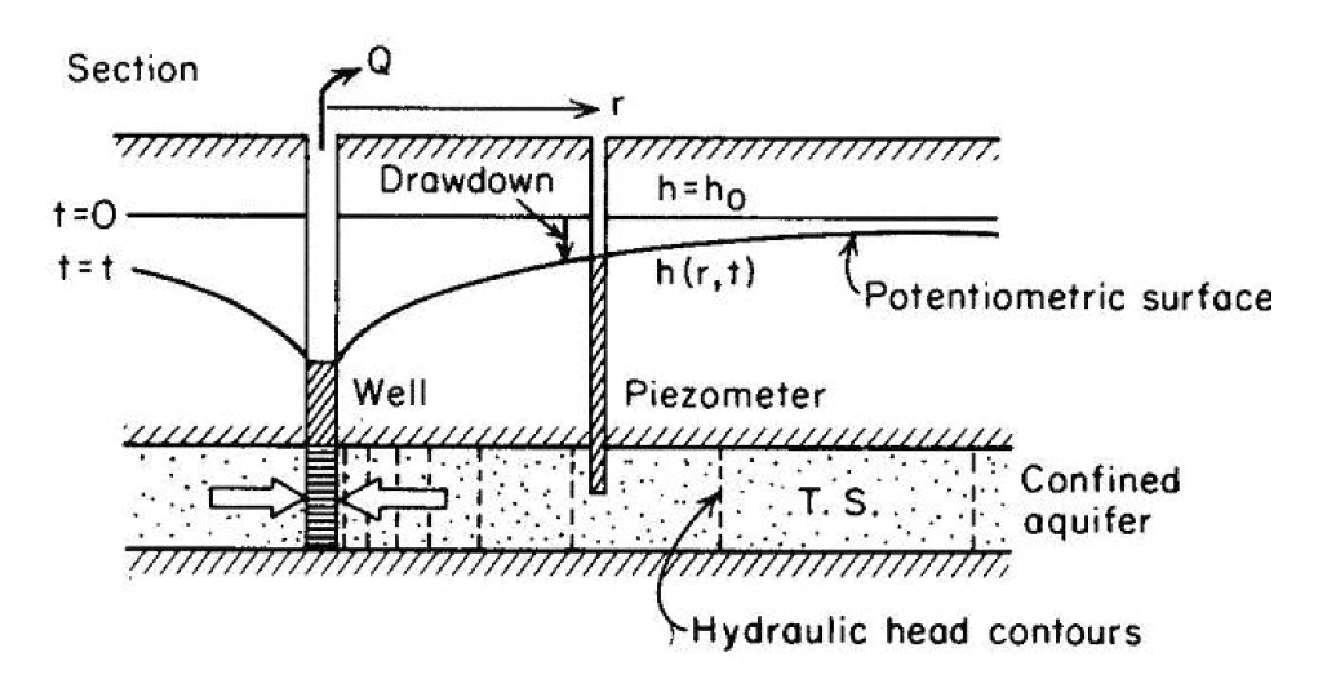
\includegraphics[width=0.5\textwidth]{C/figures/radial_flow_theiss_setup.eps}
\caption{Radial flow to a well in a confined aquifer (from Freeze and Cherry, 1979.}
\label{radial_flow_theiss_setup}
\end{figure}
The Theiss problem is used to verify the transient flow behaviour of GeoSys. Theiss (1935) presented an analytical solution for the transient drawdown in an infinite, uniform, isotropic and confined aquifer  of constant thickness (see Fig. \ref{radial_flow_theiss_setup}). The pumping well is assumed to fully penetrate the aquifer, have a neglible diameter and no well effects and to pump at a constant extraction rate. The initial hydraulic head is constant throughout the aquifer. This analytical solution is:
\begin{equation}
h_0 - h(r,t) = \frac{Q}{4\Pi T} W(\frac{r^2S}{4Tt})
\end{equation}
where $h_0$ is the initial hydraulic head [m], $h(r,t)$ is the transient hydraulic head [m] at time $t$ [s] at distance $r$ [m] from the pumping well, $Q$ is the constant extraction rate at the well [m$^3$s$^{-1}$], $S$ is the storage coefficient [-] and $T$ is aquifer transmissivity [m$^2$s$^{-1}$]. $W()$ is the Theiss well function.

The parameters used are: A model area of 1000 m times 1000 m with the well in the center, a constant thickness of 20 m, a hydraulic conductivity of 0.000578704 m/s and a storage coefficient $S_0$ of 1.000000e-005 (Caution: For the Theiss solution $S=M S_0$). This yields a transmissivity of 1000 m$^2$d$^{-1}$. Element sizes of 50 m are used, which are refined to 10 m and 2 m close to the pumping well. The pumping rate is -0.011574074 m$^{3}$s$^{-1}$, corresponding to 1000 m$^3$d$^{-1}$.

Results are shown in Figure \ref{radial_flow_theiss_top_view} in top view, also showing the grid used, and in Figure \ref{radial_flow_theiss_drawdown}, which depicts a comparison of the piezometric heads at observation points 30 m, 70 m and 100 m from the pumping well calculated by GeoSys and the analytical solution given by Theiss (1939). The correspondence is good, thus verifying radial transient flow.

\begin{figure}[htbp]
\centering
\includegraphics[width=0.5\textwidth]{C/figures/radial_flow_theiss_top_view.eps}
\caption{Radial flow to a well in a confined aquifer: Top view of the piezometric head.}
\label{radial_flow_theiss_top_view}
\end{figure}

\begin{figure}[htbp]
\centering
\includegraphics[width=0.7\textwidth]{C/figures/radial_flow_theiss_drawdown.eps}
\caption{Radial flow to a well in a confined aquifer: drawdown in the observation well, comparison to the analytical solution.}
\label{radial_flow_theiss_drawdown}
\end{figure}


\begin{table}[htbp]
\centering
\begin{tabular}{|l|l|l|}
\hline
Benchmark & Type & Path \\
\hline
\texttt{radial\_flow\_Theiss}& H &  benchmarks$\backslash$H$\backslash$radial\_flow\_Theiss  \\			
\hline
\end{tabular}
\end{table}

\subsection{Conservative Transport in radial flow}

This benchmark describes the behaviour of a conservative tracer injected in a fully penetrating well in a two-dimensional homogeneous confined aquifer.
The main purpose is to compare the numerical results of a conservative mass transport simulation without
any reactions in a radial flow field, with the approximate analytical solution for this problem that is given by Moench and Ogata (1981) and available in a computer program (LTIRD) provided by Javandel, Doughty, and Jsang (1984).

The aquifer is represented by a two-dimensional model of 300 m in both x and y direction with constant head boundary conditions at the four sides of the domain. The model is discretized in 30 rows and 30 columns with a constant width of 10 m. In order to obtain a better accuracy in the results, an area of 20 m around the injection well is further refined. The aquifer has an isotropic hydraulic conductivity K of 1.15741 $\cdot$10$^{-5}$ m s$^{-1}$, a porosity of 0.3 and injection rate Q 1.157407 $\cdot$10$^{-3}$ m$^{3}$ s$^{-1}$. Both longitudinal and transverse dispersivity have the same value  $\alpha_L$ $\alpha_T$ set to 10 m, while due to the model dimension and flow velocity, the diffusion coefficient is neglect. The physical aquifer parameters are summarized in Tab.~\ref{l_tab_benchmark_tracer_radial_flow}. The transport simulation is run for a period of 2332800 s with a time step length of 243 s.

\begin{table}[htbp]
\caption{Parameters used for benchmark HC$\backslash$radial\_flow\_transport}
\centering
\begin{tabular}{|l|l|l|}
\hline
parameter & value & unit \\
\hline
porosity $\Phi = n $  & 0.3&  --  \\			
\hline
hydraulic conductivity $K$ & 1.15741$\cdot 10^{-5}$ & ms$^{-1}$ \\ 			
\hline
injection rate $Q $ & 1.157407$\cdot 10^{-3}$ & m$^3$s$^{-1}$ \\ 	 			
\hline
storage coefficient $S$ & 0.0 & s$^{-1}$ \\
\hline
longitudinal dispersivity $\alpha_L$ & 10 &  m \\
\hline
transverse dispersivity $\alpha_T$ & 10 & m \\
\hline
total simulation time & 2332800 & s  \\
\hline
time step length  & 243 & s \\
\hline
\end{tabular}
\label{l_tab_benchmark_tracer_radial_flow}
\end{table}

\subsubsection*{Evaluation method}

Model results are compared to the approximate analytical solution from Moench and Ogata (1981).

\subsubsection*{Results}

Results of the tracer distribution along a polyline after 27 days are shown in Fig.~\ref{radial_flow_tracer_distibution} and the correspondence between anlytical solution and numerical simulation is very good.


\begin{figure}[htbp]
\centering
\includegraphics[width=0.5\textwidth]{C/figures/HC_RadialTransport_profile.eps}
\caption{Tracer distribution for radial diverging flow along a profile. Comparison of analytical solution and GeoSys/RockFlow results after 27 days of injection.}
\label{radial_flow_tracer_distibution}
\end{figure}



\begin{figure}[htbp]
\centering
\includegraphics[width=0.5\textwidth]{C/figures/HC_RadialTransport_domain.eps}
\caption{Tracer distribution for radial diverging flow in top view. Isolines of tracer concentration from GeoSys/RockFlow results after 27 days of injection.}
\label{radial_flow_tracer_distibution}
\end{figure}


\begin{table}[htbp]
\centering
\begin{tabular}{|l|l|l|}
\hline
Benchmark & Type & Path \\
\hline
\texttt{radial\_flow\_transport}& HC &  benchmarks$\backslash$C$\backslash$radial\_flow\_transport  \\			
\hline
\end{tabular}
\end{table}


\section{Reactive Transport}


\subsection [Xylene degradation (1D)]{1D reactive transport: Xylene degradation with multiple monod kinetics, exchange kinetics and biomass growth}
\label{l_s_benchmark_1d_xylene_deg}

This benchmark describes the reactive transport of xylene in a homogeneous aquifer. The main purpose is to document the ongoing reactions, which are xylene degradation under aerobic, sulfate reducing and iron reducing conditions, considering growth of the respective biomasses. Also included is the rate limited exchange of iron goethite into bioavailable iron. The aquifer is represented by a one-dimensional model of 50 m length in the x-direction and 1 m in the y-and z directions, respectively. The model is discretized by 100 line elements of constant 0.5 m length in x direction. With an isotropic hydraulic conductivity K of 2.13 $\cdot$10$^{-3}$ m s$^{-1}$, a porosity of 0.24 and a hydraulic gradient I of 1.3$\cdot$10$^{-4}$, the steady state transport velocity va is 0.1 m d$^{-1}$. Longitudinal dispersivity  $\alpha_L$ is set to 0.25 m, the diffusion coefficient $D_a$ is set to 1.0$\cdot$10$^{-9}$ m$^2$ s$^{-1}$. The physical aquifer parameters are summarized in Tab.~\ref{l_tab_benchmark_1d_xylene}. The transport simulation is run for a period of 1000 d with a time step length of 5 d.

The model aquifer has a length of 50 m in the x-direction, 1 m in the y-direction and 1 m in the z direction. The whole domain is discretized into 100 line elements with a constant x and y dimension of 1 m.
The aquifer is assumed to have a homogeneous and isotropic hydraulic conductivity. Using a gradient of 1.23 $\cdot$10$^{-4}$ and a porosity of 0.24 produces a steady state transport velocity of 0.10 m d$^{-1}$.

Xylene degradation is simulated according to the typical redox sequence.


\begin{table}[htbp]
\caption{Parameters used for benchmark HC$\backslash$1d\_xylene\_degradation }
\centering
\begin{tabular}{|l|l|l|}
\hline
parameter & value & unit \\
\hline
porosity $\Phi = n $  & 0.24 &  --  \\			
\hline
matrix volume fraction $VOL_MAT $  & 0.75 &  --  \\			
\hline
biomass volume fraction $VOL_BIO $  & 0.01 &  --  \\			
\hline
hydraulic conductivity $K$ & 2.13$\cdot 10^{-3}$ & ms$^{-1}$ \\
\hline
storage coefficient $S$ & 0.0 & s$^{-1}$ \\
\hline
solid density $\rho_s$ & 2000 &  kg$\cdot m^{-3}$ \\
\hline
density of water $\rho_w$ & 1000 & kg$\cdot m^{-3}$ \\
\hline
viscosity water $\eta$ & 0.001 & Pa$\cdot s$ \\
\hline
longitudinal dispersivity $\alpha_l$ & 0.25 & m \\
\hline
component diffusion coefficient $D$ & 1.0$\cdot 10^{-9}$ & m$^2$s$^{-1}$ \\
\hline
\end{tabular}
\label{l_tab_benchmark_1d_xylene}
\end{table}

\subsubsection*{Evaluation method}

Model results are compared an older version of GeoSys/RockFlow.

\subsubsection*{Results}

Results of the simulation are shown in Fig.~\ref{profiles_xylene_degradation} for xylene, the electron acceptors oxygen and sulfate, as well as for the biomass of the aerobic microorganisms, the sulfate reducers and the iron reducers simulation time steps of 100 days.
For simulation time t $<$ 500~d, one can see the advancing xylene front, a reduction of xylene concentrations is only visible for later times, when xylene concentrations reduce to about 90\% of the inflow concentration. Also shown is the increasing consumption of oxygen with time, accompanied by the growth of the aerobic reducers at the inflow (left) end of the model area. After approximately 800~d, oxygen concentrations in the inflowing groundwater are reduced to almost zero within the first 20~m of the aquifer. Sulfate reducers initially decay from their initial amount, as growth is inhibited throughout the column by the still high concentrations of oxygen. Once oxygen is used up, however, sulfate reducers start to grow downstream of the oxygen reducers and sulfate concentrations in the groundwater reduce accordingly. The iron reducers decay from their initial values and start to grow only for late times t $>$ 80~d and x $>$ 30~m, as xylene degradation from iron reduction is inhibited by both, oxygen as well as sulfate, which is still present in concentrations larger than the inhibition concentration for iron reducers. Accordingly, the spatial distribution of bioavailable iron is still almost uniform throughout the aquifer.
%Figure 2 shows the slow temporal decrease of goethite concentrations and the corresponding increase in bioavailable iron concentrations resulting from the slow transfer kinetics.


\begin{figure}[htbp]
\centering
\includegraphics[width=0.9\textwidth]{C/figures/profiles_xylene_degradation.eps}
\caption{Profiles of oxygen, sulfate and xylene (top row, from left) and  aerobic reducers, sulfate reducers and iron reducers at different times during the 1000 d simulation period.}
\label{profiles_xylene_degradation}
\end{figure}


\begin{table}[htbp]
\centering
\begin{tabular}{|l|l|l|}
\hline
Benchmark & Type & Path \\
\hline
\texttt{1d\_xylene\_degradation}& HC &  benchmarks$\backslash$C$\backslash$1d\_xylene\_degradation  \\			
\hline
\end{tabular}
\end{table}




\subsection[Competition of TCE- and cis-DCE-degradation for zero valent iron surface (1D)]{1D reactive transport: Competition of TCE- and cis-DCE-degradation for the zero valent iron surface}
\label{l_s_benchmark_1d_TCEonIon}

This example simulation demonstrates the use of GeoSys/RockFlow for simulation of multi-species kinetic reactions. The reaction system was set up by D. Schäfer and published in Schäfer et al. (2003) (Schäfer, D., R. Köber and A. Dahmke (2003): Competing TCE- and cis-DCE-degradation kinetics by zero-valent iron - experimental results and numerical simulation. Journal of Contaminant Hydrology, 65(3-4): 183-202). Further, it was used for model verification of the newly implemented and developed kinetic reaction module in GeoSys/RockFlow. The example considers flow in a one-dimensional column of 1 m length, resembling the thickness of a reactive iron barrier perpendicular to the flow direction. It involves 19 species and and 16 different geochemical reactions, both first-order degradation reactions of adsorbed substances and kinetic sorption reactions of the langmuir-type, considering competition for the available sorption sites.

The model set up consists of a 1d column with saturated ground water flow with a darcy velocity of 5.0$\cdot$ 10$^{-4}$ m d$^{-1}$ from left to right. Geochemical species are added to the inflowing water, and their sorption and degradation behavior is modeled. For a complete description of input parameters see the paper by Schfer et al. (2003). Every degradation reaction follows a Langmuir-Hinshelwood-Hougen-Watson kinetics with a limited number of sites for the adsorption and desorption of chlorinated hydrocarbons on the reactive iron surface. Since all the reactive substances involved have to adsorb onto the reactive iron surface in order to be degraded, a competition for the surface sites occurs. This competition has been investigated in column studies and the observed concentration profiles were simulated with the numerical model TBC (Schfer et al., 2003).



\subsubsection*{Evaluation method}

Model results are compared an older version of GeoSys/RockFlow, which was compared to the original TBC simulations.

\subsubsection*{Results}

Results of the simulation are shown in Fig.~\ref{profiles_TCEonIon}, where profiles of the dissolved species are shown. TCE and cis-DCE are added to the inflowing water. They compete for the sorption sites, and when sorbed degrade according to a first order degradation reaction. The retardation of the reactive species compared to the conservative tracer \texttt{mobile} is clearly visible. Also, just downstream of the concentration decrease of TCE or cis-DCE, the degradation products ethane and C4-containing molecules increase. These species are again mobile and are transported with the water, so an instationary behaviour is observed in Fig.~\ref{profiles_TCEonIon}.

\begin{figure}[htbp]
\centering
\includegraphics[width=0.9\textwidth]{C/figures/1d_TCEonIon.eps}
\caption{Concentration profiles of TCE, trans-DCE, cis-DCE, 1,1-DCE, Acetylene, chloroacetylene, C4, VC, ethene and ethane as well as the concervative tracer mobile after 50 d simulation time.}
\label{profiles_TCEonIon}
\end{figure}


\begin{table}[htbp]
\centering
\begin{tabular}{|l|l|l|}
\hline
Benchmark & Type & Path \\
\hline
\texttt{1d\_TCEonIon}& HC &  benchmarks$\backslash$C$\backslash$1d\_TCEonIon  \\			
\hline
\end{tabular}
\end{table}




\input{C/isofrac}
%

\subsection{Kinetic phase transfer NAPL - water}

In this benchmark, a simplified two-phase (NAPL-water) flow model is coupled with mass transport and kinetic dissolution of the NAPL phase. The NAPL here is assumed to be in residual saturation and hence immobile, while the water phase is mobile and transports the dissolved species. The PS\_GLOBAL model is used for the simulation of the two-phase flow process. Two simple tests first are used to verify the correctness of the flow field and the coupling of flow and transport processes for all element types. The kinetic dissolution model is tested by comparison to an analytical solution.

\subsubsection{Flow in presence of a residual immobile NAPL phase}
\label{NAPL_diss_BM_flow}

Groundwater flow in presence of a residual NAPL phase is simulated in a one-dimensional model of 50 m length in $x$ direction. The residual NAPL is present as blobs (or ganglia) in a five m long zone between $x$ = 5 - 10 m from the left hand side boundary of the model and has a saturation $S_n$ = 0.10. Accordingly, water saturation $S_w$ = 0.90 in this zone, while $S_w$ = 1.0 elsewhere. Water phase relative permeability $k_{r_w}$ [-] is described using the Brooks-Corey model
\begin{equation}
k_r = \left(S_{eff}\right)^{\frac{2+3\lambda}{\lambda}}
\label{eq_brooks-corey_krel}
\end{equation}
with $\lambda$ $= 0.386$ [-] as an empirical parameter, and is reduced to a value of 0.625 in the NAPL zone. Water effective saturation is given by
\begin{equation}
S_{eff} = \frac{S_w-S_{r_w}}{S_{s_w}-S_{r_w}}
\label{eq_Seff_brooks-corey}
\end{equation}
NAPL immobility is achieved by setting the NAPL residual saturation $S_{r_n} > S_n$. NAPL phase relative permeability accordingly is 0.0 throughout the model domain.

As the NAPL is in residual saturation and thus immobile, and dissolution reactions are not considered at the moment, $S_n$, $S_w$ and $k_{r_w}$ remain temporally constant. Constant pressure boundary conditions are used on the left and right hand side model boundary, which induce an average hydraulic gradient of 0.01. Linear, quadrilateral, hexahedral, triangular, prismatic as well as tetrahedral elements are used for the spatial discretization of the model. The size of the elements is 1/3 m in $x$ direction in each case, i.e. for the 1D line element model, 150 elements are used. Model parameters for the simulation are summarized in Tab.~\ref{l_tab_benchmark_1d_NAPLdiss_hydr}.

\begin{table}[htbp]
\caption{Model parameters used for the test case. }
\centering
\begin{tabular}{|l|l|l|}
\hline
parameter & value & unit \\
\hline
model length $x$ &	50	& m  \\			
\hline
model length $y$ &	1.0	& m  \\		
\hline
model length $z$ &	1.0	& m  \\		
\hline
element length $x$ &	0.333	& m  \\		
\hline
porosity $n$  & 0.25 &  --  \\			
\hline
permeability $k$  & 1.54249$\cdot$10$^{-11}$ &  m$^2$  \\			
\hline
tortuosity $\tau$ & 1.0  & -- \\
\hline
residual water saturation $S_{r_w}$ & 0.2 & -- \\
\hline
saturated water saturation $S_{s_w}$ & 1.0 & -- \\
\hline
residual NAPL saturation $S_{r_n}$ & 0.2 & -- \\
\hline
saturated NAPL saturation $S_{s_n}$ & 0.95 & -- \\
\hline
$\lambda$ (Brooks-Corey parameter) & 3.86 & -- \\
\hline
density of water $\rho_w$ & 1000 & kg  m$^{-3}$ \\
\hline
viscosity water $\eta$ & 0.001 & Pa s \\
\hline
initial $S_w$ ($x<$5 m \& $x>$10 m, $t$=0)  & 1.0 & -- \\
\hline
initial $S_w$ ($x>$5 m \& $x<$10 m, $t$=0)  & 0.90 & -- \\
\hline
initial $S_n$ ($x<$5 m \& $x>$10 m, $t$=0)  & 0.0 & -- \\
\hline
initial $S_n$ ($x>$5 m \& $x<$10 m, $t$=0)  & 0.10 & -- \\
\hline
initial water pressure ($x$, $t$=0) & 98067.0  & Pa \\
\hline
water pressure ($x$=0, $t$) &  98067.0 & Pa \\
\hline
water pressure ($x$=50, $t$) & 93163.65 & Pa \\
\hline
\end{tabular}
\label{l_tab_benchmark_1d_NAPLdiss_hydr}
\end{table}

The hydraulic 1D model is compared against an equivalent single (water) phase groundwater flow model, in which a zone of reduced hydraulic permeability is introduced at the position of the NAPL zone (i.e. between $x$ = 5 m and $x$ = 10 m), with $K$ = 9.64056$\cdot10^{-12}$ m$^2$, which corresponds to $K$ in the NAPL zone of the two-phase model.

Fig.~\ref{profiles_pressure_NAPLflow} shows the numerical solution of the pressure distribution after a time step of 21600 s. The pressure gradient in the water phase is uniform up to $x$ = 5 m, increases in the NAPL zone due to the reduction of permeability and decreases again for $x>$ 10 m. Simulations for all element types show identical pressure distributions. The individual graphs therefore cannot be distinguished in Fig.~\ref{profiles_pressure_NAPLflow}.

\begin{figure}[htbp]
\centering
\includegraphics[width=0.6\textwidth]{C/figures/NAPL_diss_pressure.eps}
\caption{Water phase pressure distribution along the 1D model for different element types and two equivalent single phase groundwater flow models with reduced hydraulic permeability between $x$ = 5 m and $x$ = 10 m.}
\label{profiles_pressure_NAPLflow}
\end{figure}

The pressure distribution of the groundwater flow model (blue dashed graph) matches the two-phase model pressure distribution almost exactly, although some very small discrepancies exist at the transition zones between NAPL zone and the fully water saturated domain. These differences are due to the handling of the discontinuous phase saturation distribution at the boundaries of the NAPL zone, i.e. at $x$ = 5 and $x$ = 10 m. In the two-phase model, for elements in the direct vicinity of the NAPL zone element matrices are calculated assuming a saturation interpolated from the element nodes saturation values, which results in $S_n >$ 0, $S_w <$ 1 and $k_{r_w} <$ 1, and the observed deviation from the pressure distribution of the groundwater flow model. In Fig.~\ref{profiles_pressure_NAPLflow} the black dash-dotted graph shows the pressure distribution from a modified groundwater flow model, where a hydraulic permeability of $K$ = 1.229174$\cdot10^{-11}$ m$^2$ was assigned to the two elements in the direct vicinity of the NAPL zone, which corresponds to the reduced water phase permeability of these elements in the two-phase model. In this case the pressure distribution matches the two-phase model results exactly.

\subsubsection{Conservative transport in presence of a residual immobile NAPL phase}
\label{NAPL_diss_BM_transport}

This test is based on the previously presented simulation, which is extended for a conservative mass transport process by infiltration of a non-reactive tracer at a constant concentration of 1.0 at the left hand side model boundary, i.e. at $x$ = 0 m, for a period of 500 time steps of 21600 s. Longitudinal dispersivity  $\alpha_L$ = 0.5 m, the aqueous diffusion coefficient D$_{aq}$ = 1$\cdot10^{-9}$ m$^2$ s$^{-1}$. All other model parameters are kept identical to the previous test case.

In contrast to transport in fully water saturated media, in the presence of a NAPL phase transport takes place in a reduced volume $nS_w$, where $S_w$ is taken from the flow step (and hence from the old time level)
\begin{equation}
    n S_w\frac{\partial C_{w,i}}{\partial t} + \textbf{\textrm{q}}_w \nabla C_{w,i} - \nabla \cdot\left( nS_w\textbf{\textrm{D}}_i \nabla C_{w,i} \right)+nS_wQ_{C_{w,i}}=0
    \label{eq_trans_water_NAPLdiss}
\end{equation}
where $C_{w,i}$  [M L$^{-3}_{water}$] is the concentration of component $i$ in groundwater, \textbf{q}$_w$ the Darcy velocity [L T$^{-1}$] and \textbf{D}$_i$ the dispersion tensor [L$^2$T$^{-1}$]. As the NAPL phase is stationary and residual, its phase velocity is zero and components present in the NAPL phase remain immobile. The corresponding transport equation hence only consists of the source term from NAPL dissolution:
\begin{equation}
    n S_n\frac{\partial C_{w,j,i}}{\partial t} +nS_nQ_{C_{n,j,i}}=0
    \label{eq_trans_NAPL_NAPLdiss}
\end{equation}
As the source term in \ref{eq_trans_NAPL_NAPLdiss} is explicitly accounted for in the computation of the exchange processes (see below), a solution of \ref{eq_trans_NAPL_NAPLdiss} on the model grid is not necessary.

The 1D transport model is compared against an equivalent single (water) phase groundwater flow and transport model. Fig.~\ref{profiles_tracer_NAPLtransp} presents breakthrough curves of the tracer at $x$ = 15 m, i.e. 5 m downgradient from the NAPL zone, for all element types and the two equivalent groundwater flow models, in which in addition to the permeabilities also porosities were matched with the effective porosities of the two-phase model. Results for all element types compare well, although a plot of breakthrough concentrations on a logarithmic scale (right diagram) reveals small differences between different element types for early moments of the two-phase simulation and small breakthrough concentrations. In comparison, the tracer breakthrough curve for the equivalent groundwater flow model matches the results of the two-phase model precisely.

\begin{figure}[htbp]
\centering
\includegraphics[width=1\textwidth]{C/figures/NAPL_diss_BTC.eps}
\caption{Tracer breakthrough concentrations in the 1D model at $x$ = 15 m downgradient from the left hand side model boundary for different element types and two equivalent single phase groundwater flow models with reduced hydraulic permeability between $x$ = 5 m and $x$ = 10 m. Left diagram: linearly scaled concentrations; right diagram: logarithmic concentrations.}
\label{profiles_tracer_NAPLtransp}
\end{figure}


\subsubsection{Dissolution of a multi-component NAPL phase}
\label{NAPL_diss_BM_diss}

The kinetic dissolution model is validated against the Hansen and Kueper analytical solution ~\cite{HanKue:07}. The  Hansen and Kueper model ~\cite{HanKue:07} model was developed to quantify the temporally changing composition of a residual multi-component NAPL body in moving groundwater and the consequent changes of the NAPL constituents concentrations in the surrounding groundwater. It is suited for both, pooled configurations and residual NAPL in blob geometries and - as any analytical model - is based on a number of simplifying assumptions:
\newenvironment{bulletpopints}{\begin{itemize}}{\end{itemize}}
\begin{bulletpopints}
 \item The model predicts the NAPL composition as well as aqueous phase concentrations at the downstream end of the NAPL source zone (Fig.~\ref{fig_HKAS_concept}).
\item  Intra-NAPL diffusion is fast in relation to phase partitioning.
\item  For pools the local equilibrium assumption is employed, i.e. inter-phase mass transfer is faster than solute transport away from the NAPL.
\item  Within a zone of residual NAPL, NAPL saturation and mixing are sufficient to allow the assumption of a uniform concentration composition at the downstream end of the source zone (perfectly mixed source), which follows Raoult's law (global equilibrium assumption).
\item  The component composition of the NAPL is spatially invariant at a particular instant in time.
\item  Dissolution kinetics are fast at all times (equilibrium dissolution).
\item  NAPL saturation, effective porosity and water flux through the source are constant in time.
\end{bulletpopints}

The Hansen and Kueper model ~\cite{HanKue:07} for a residual NAPL source zone was represented as a one-dimensional numerical model of 50 m length in $x$ direction using linear finite elements and a spatial discretization $\Delta x$ = 1/3 m, i.e. the same model geometry as in the previous two test cases is used here. The assumption of a perfectly mixed residual NAPL source zone is represented as a zone of blobs at a single node of the finite element mesh directly downgradient of the left hand side model boundary at $x$ = 1/3 m (Fig.~\ref{fig_HKAS_FEM}).

\begin{figure}[htbp]
\centering
\includegraphics[width=0.9\textwidth]{C/figures/H&K_concept.eps}
\caption{Conceptualization of the Hansen and Kueper (2007) analytical solution: Example of a three component residual NAPL source zone in a moving groundwater body and source emission.}
\label{fig_HKAS_concept}
\end{figure}

\begin{figure}[htbp]
\centering
\includegraphics[width=0.9\textwidth]{C/figures/H&K_concept_FEM.eps}
\caption{Representation of the Hansen and Kueper (2007) analytical solution in a numerical model. The red dot represents the position of the NAPL blob zone in the linear finite element mesh.}
\label{fig_HKAS_FEM}
\end{figure}

The temporally constant flux through the NAPL source is induced by source terms of $q_{in} =-q_{out} = 1.157\cdot10^{-6}$ m s$^{-1}$ at the left and right hand side model boundaries, respectively (Fig.~\ref{fig_HKAS_FEM}). The NAPL consists of the three chlorinated hydrocarbon (CHC) species perchloroethene (PCE), trichloroethene (TCE) and tetrachloromethane (TCM). Accordingly, three immobile NAPL species plus three corresponding mobile species are defined in the model. Tab.~\ref{l_tab_benchmark_1d_HKAS_compprop} lists physicochemical parameters and initial amounts or concentrations, respectively, assumed for the three immobile NAPL species in this simulation.

\begin{table}[htbp]
\caption{Physicochemical properties and initial concentrations of the immobile NAPL species.}
\centering
\begin{tabular}{|l|l|l|l|l|}
\hline
parameter & Unit & PCE & TCE & TCM \\
\hline
molar weight & [kg mol$^{-1}$] & 0.166 & 0.131 & 0.154	\\
\hline
molar density & [mol m$^{3}$] & 9770.800 & 11111.100 & 12395.300\\	
\hline
max. aq. solubility & [mol/m$^{3}$] & 1.150 & 10.650 & 72.860\\
\hline
concentration & [mol/m$^{3}_{REV}$] & 122.140 & 111.110 & 30.990\\
\hline
volume per m$^{3}_{REV}$ & [m$^3$] & 0.013 & 0.010 & 0.003\\
\hline
mass per m$^{3}_{REV}$ & [kg] & 20.254 & 14.599 & 4.767\\
\hline
\end{tabular}
\label{l_tab_benchmark_1d_HKAS_compprop}
\end{table}

Corresponding mobile species in the aqueous phase share the same physicochemical properties. Initial concentrations at the second node of the mesh (i.e. at the NAPL source position) correspond the equilibrium concentrations according to Raoult's law and the initial moles of the immobile NAPL components, i.e. C$_{PCE}$ = 0.532, C$_{TCE}$ = 4.478 and C$_{TCM}$ = 8.545 mol m$^{-3}$, respectively. Elsewhere, initial concentrations (as well as upstream boundary conditions) are set to C = 1.0$\cdot10^{-10}$ mol m$^{-3}$. In the NAPL source S$_n$ = 0.10 and S$_w$ = 0.90, accordingly, while S$_w$ = 1.0 and S$_n$ = 0.0 elsewhere. Water phase relative permeability k${_{r_w}}$ [-] is described by the Brooks-Corey model (see above). Other model parameters (and those deviating from the model setup of the previous two test cases) are summarized in Tab.~\ref{l_tab_benchmark_1d_HKAS_hydr}.

\begin{table}[htbp]
\caption{Model parameters used for benchmark ~\ref{NAPL_diss_BM_diss} }
\centering
\begin{tabular}{|l|l|l|}
\hline
parameter & value & unit \\
\hline
longitudinal dispersivity  $\alpha_L$  & 0.09 &  m\\
\hline
mean grain diameter $d_{50}$  & 0.001 &  m\\
\hline
Sherwood factor $SF$  & 1.15 &  --\\
\hline
Reynolds exponent $RE$  & 0.654 &  --\\
\hline
Schmidt exponent $SE$  & 0.486 &  --\\
\hline
interfacial area $a$  & 5000.0 &  m$^2$ m$^{-3}_{REV}$\\
\hline
\end{tabular}
\label{l_tab_benchmark_1d_HKAS_hydr}
\end{table}



Mass transfer between the NAPL and the aqueous phase for individual components $i$ is described by Fick's 1st law
\begin{equation}
    \frac{\partial M}{\partial t} =  k a \left( C_{w,i}^{sat}  -  C_{w,i}  \right)
    \label{eq_mass_transfer}
\end{equation}
The rate of mass transfer [M T$^{-1}$] depends mainly on the concentration difference between the equilibrium concentration [M L$^{-3}$] and the actual concentration [M L$^{-3}$] in the water phase as well as on the mass transfer parameter $k$ [L T$^{-1}$] and the water-NAPL contact area $a$ [L$^2$]. For NAPL mixtures $C^{sat}_{w,i}$ is calculated according to Raoult's law. The mass transfer coefficient $k$ can be determined by
 \begin{equation}
k = SF \left( \frac{\rho_w v_a d_{50}}{\mu_w}  \right)^{RE}  \left( \frac{\mu_w }{D_{aq} \rho_w}  \right)^{SE} \frac{D_{aq}}{d_{50}}
    \label{eq_mass_transfer_coefficient}
\end{equation}
where $d_{50}$ [L] is the mean grain size diameter, $D_{aq}$ [L$^2$ T$^{-1}$] is the coefficient of diffusion in water, $SF$  [-] is the Sherwood-factor and $RE$ [-] and $SE$ [-] are the Reynolds- and Schmidt-exponents, as the two terms in brackets are termed Reynolds- and Schmidt-numbers, respectively. The interfacial area $a$ is set to a constant and very large value of 5000.0 m$^2$ m$^{-3}_{REV}$ in order to guarantee fast (i.e. quasi equilibrium) NAPL dissolution kinetics, as assumed by the analytical solution. The simulation is run for a period of 1.08$\cdot10^{-8}$ s with 10000 time steps of 10800.0 s length.

\subsubsection*{Results}

Fig.~\ref{fig_HKAS_vs_GeoSys} presents the amounts of the the three immobile species PCE, TCE and TCM in the NAPL phase (left diagram) and the corresponding aqueous phase concentrations (i.e. the source emission; right diagram) as functions of time. Full lines are for the analytical solution, while symbols represent results of the numerical simulation. The agreement is excellent over a concentration range of several orders of magnitude. TCM, which has the highest pure phase aqueous solubility is depleted fastest from the source. TCE and especially PCE depletion requires significantly longer time periods. Aqueous phase concentrations of PCE drop almost instantaneously, once the remaining amount of PCE in the NAPL falls below a threshold of 0.28 mol.

\begin{figure}[htbp]
\centering
\includegraphics[width=0.9\textwidth]{C/figures/H&K_ASvsGS.eps}
\caption{Total amounts of PCE, TCE and TCM in the NAPL phase (left diagram) and corresponding aqueous phase concentrations at the downgradient source zone margin (right diagram) as functions of time; full lines: analytical solution of Hansen and Kueper (2007), symbols: GeoSys simulation results.}
\label{fig_HKAS_vs_GeoSys}
\end{figure}


\begin{table}[htbp]
\centering
\begin{tabular}{|l|l|l|}
\hline
Benchmark & Type & Path \\
\hline
\texttt{1D\_TPF\_resS\_flow}& HC &  inputfiles$\backslash$benchmarks$\backslash$1D\_NAPL-diss\_flow  \\			
\hline
\texttt{1D\_TPF\_resS\_transport}& HC &  inputfiles$\backslash$benchmarks$\backslash$1D\_NAPL-diss\_transport  \\			 \hline
\texttt{1D\_TPF\_resS\_dissolution}& HC &  inputfiles$\backslash$benchmarks$\backslash$1D\_NAPL-diss\_dissolution \\			 \hline
\end{tabular}
\end{table}



%\section{Biodegradation}

%\subsection{Advective dispersive diffusive transport and zero order kinetic degradation of PCE}
%\subsection{Advection + dispersion + diffusion 1st order kinetic degradation of PCE}
%\subsection{Advective dispersive diffusive transport and 2nd order kinetic degradation}
%\subsection{Advective dispersive diffusive transport and degradation following a Monod kinetic}
%\subsection{Advective dispersive diffusive transport and degradation following a multiplicative Monod kinetic}
%\subsection{Advection + dispersion + 1st order kinetic degradation + linear sorption of Metalaxyl}
%\subsection{Influence of sorption reactions on contaminant transport and degradation rates}
%\subsection{Advective dispersive diffusive transport, degradation and microorganism growth}

%\subsection{Competition of TCE- and cis-DCE-degradation for the zero valent iron surface}
%\subsection{Microbial xylene degradation}
%\subsection{Microbial xylene degradation via sulfate reduction}

\subsection[Degradation network (1D)]{1D reactive transport: degradation of organic contaminants in a
sand column experiment by five bacterial groups forming a degradation network}
\label{l_s_benchmark_1d_network}

%Column experiments are often used to study the degradation of organic
%contaminants in the saturated groundwater zone.

The Biogeochemical Reaction Network
Simulator~(BRNS,~\cite{Aguilera2005,Regnier2002}) is coupled to GeoSys
following a sequential non-iterative operator splitting scheme yielding the
reactive transport model GeoSysBRNS. The technical
coupling is sketched in Fig.~\ref{fig:GeoSysBRNSSetup}.

\begin{figure}[h!]
\centering
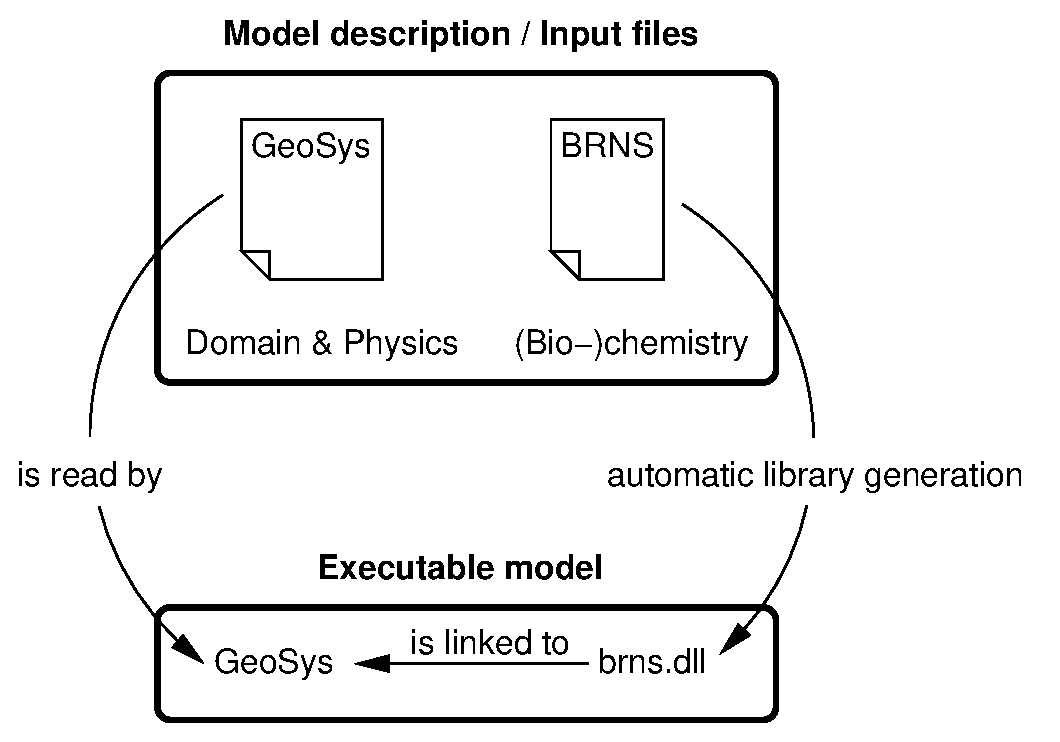
\epsfig{file=C/figures/GeoSysBRNSSetup.eps,width=8cm}
\caption{
The setup of GeoSysBRNS. The model description is divided into two parts: the
model domain definition, physical parameters, hydrogeological flow, and
discretization parameters in GeoSys format, and the description of the coupled
(bio-)chemical reaction processes in BRNS format. The latter is compiled into a
problem specific library that is accessed by GeoSys at runtime.
}
\label{fig:GeoSysBRNSSetup}
\end{figure}

\subsubsection*{The Model}

An experimental study by~\cite{Gunten1993} has been used to validate the
reactive transport models TBC~\cite{Schaefer1998b} and the stand-alone 1D
version of BRNS~\cite{Thullner2005}.  Both models could reproduce the
experimental data set. Here, we use the same simulation scenario to validate
GeoSysBRNS and compare simulation results to BRNS results.

In the example referred to as ``Scenario 1'' in~\cite{Thullner2005}, a sand
column of 29 centimeters length is constantly flushed with water containing
lactate as electron donor, and oxygen, nitrate, and sulfate as terminal
electron acceptors~(TEAs). Manganese and iron oxyhydroxides are bound to the
sand matrix in solid phases and act as two additional TEAs. Five distinct
microbial groups, which catalyze the reduction of each TEA to sustain their
growth, are considered in the model. The experimental results suggest that
lactate is concomitantly mineralized into dissolved inorganic carbon~(DIC) and
fermented to acetate and proprionate, with the latter being further oxidized
into DIC.  In addition to these microbial degradation pathways, reactive
species concentrations are influenced by a set of abiotic
reactions~(Fig.~\ref{fig:sandnetwork}).  The complete reaction network of the
model consists of 21 mobile and 18 immobile reactive species. The dynamics of
the system is determined by 24 kinetically controlled chemical reactions and
nine equilibrium reactions describing acid base dissociations.

\begin{figure}[h!]
$\bullet$ phase exchange (matrix, biophase, pore water)\\
$\bullet$ oxidation of sulfide by Fe(III)\\
$\bullet$ precipitation and dissolution of calcite and\\
Fe(II) minerals\\
$\bullet$ acid-base reactions for carbonates, sulfides,\\
lactate, propionate, acetate

\vspace{-2.75cm}
\hspace{8cm}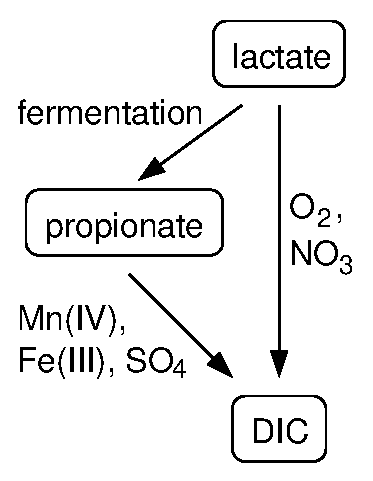
\epsfig{file=C/figures/GeoSysBRNSSandNetwork.eps,width=3.0cm}
\caption{
Modeling organic carbon degradation in a sand column experiment.  Coupled
abiotic processes considered in the model~(left), and microbial degradation
pathways with corresponding TAEs~(right).
}
\label{fig:sandnetwork}
\end{figure}

\subsubsection*{Evaluation method}

The coupling of the BRNS to GeoSys is shown to be correct by comparing
simulation results of GeoSysBRNS to BRNS results~\cite{Centler2009}.

\subsubsection*{Results}

We simulate the experiment with GeoSysBRNS using two spatial resolutions and
three different temporal resolutions per spatial setting, ensuring Courant
numbers smaller than 1.0 in all cases.  As in previous
studies~\cite{Thullner2005,Schaefer1998b}, we choose 48 days as the target
time for comparing the results of the coupled model to those obtained with the
BRNS model using the same set of spatio-temporal resolution settings.  At this
target time, the system is still in the transient phase. 

The simulation results of GeoSysBRNS and BRNS agree very well for all 39
reactive species at the highest spatial and temporal resolution~(see selected
species in Figs.~\ref{fig:columnresultsfine1},~\ref{fig:columnresultsfine2}).
Decreasing the spatial resolution leads to slightly different results, with the
coupled model generally staying closer to the high resolution result than the
stand-alone version of
BRNS~(Figs.~\ref{fig:columnresultsfine1},~\ref{fig:columnresultsfine2}).

When the time step size is increased, the numerical results of both models
diverge from the high resolution result~(Fig.~\ref{fig:columnresults}).  While
increasing the time step from 4 s to 43.2 s does not lead to significant
changes for both models and both spatial resolutions, a noticable deviation is
observed when the time step size is further increased to 108 s for the high,
and to 216 s for the low spatial resolution.  For these larger time step sizes,
the results of GeoSysBRNS are again generally closer to the high resolution
result than the BRNS solutions.  The observed differences can be attributed to
the different numerical schemes used by BRNS~(finite differences) and
GeoSysBRNS~(finite elements). Further details of the GeoSysBRNS and its
performance can be found in~\cite{Centler2009}.


\begin{table}[h!]
\centering
\begin{tabular}{|l|l|l|}
\hline
Benchmark & Type & Path \\
\hline
\texttt{1d\_degradation\_network}& C & benchmarks$\backslash$C$\backslash$1d\_degradation\_network \\
\hline
\end{tabular}
\end{table}

\begin{figure}[h!]
\centering
\epsfig{file=C/figures/GeoSysBRNSfinest_la_pro_ac.eps,angle=270,width=11cm}\\
\epsfig{file=C/figures/GeoSysBRNSfinest_biomass.eps,angle=270,width=11cm}
\caption{
Comparison of simulation results obtained with BRNS~(lines) and
GeoSysBRNS~(symbols): organic species~(top) and all five bacterial
groups~(bottom) at day 48 using the highest temporal resolution~($\Delta$t=4 s)
and two spatial resolutions. 
}
\label{fig:columnresultsfine1}
\end{figure}

\begin{figure}[h!]
\centering
\epsfig{file=C/figures/GeoSysBRNSfinest_nit_sul_mn.eps,angle=270,width=11cm}\\
\epsfig{file=C/figures/GeoSysBRNSfinest_s_fe.eps,angle=270,width=11cm}
\caption{
Comparison of simulation results obtained with BRNS~(lines) and
GeoSysBRNS~(symbols): inorganic species at day 48 using the highest temporal
resolution~($\Delta$t=4 s) and two spatial resolutions. 
}
\label{fig:columnresultsfine2}
\end{figure}

\begin{figure}[h!]
\centering
\epsfig{file=C/figures/GeoSysBRNSla_pro_ac.eps,angle=270,width=11cm}\\
\epsfig{file=C/figures/GeoSysBRNSla_pro_ac_fine.eps,angle=270,width=11cm}
\caption{
Comparison of simulation results obtained with BRNS~(lines) and
GeoSysBRNS~(symbols) at day 48 using two spatial resolutions~(top:
$\Delta$x=3.9mm, bottom: $\Delta$x=1.45mm) and different time step sizes for
lactate, proprionate, and acetate.
}
\label{fig:columnresults}
\end{figure}

\clearpage


\subsection{Mixing Controlled Bioreactive Transport (2D)}
\input{C/monod2d}
